\documentclass[journal,10pt]{IEEEtran}
\usepackage{fontspec}
\setmainfont{Times New Roman}
\setmonofont{Consolas}
\usepackage{amsmath,amssymb,amsfonts}
\usepackage{graphicx}
\graphicspath{{../}{../04_Figures_and_Assets/}{D:/APAL-Dynamic-v4/docs/APAL_HGP_PPO_Journal_Manuscript/}}
\usepackage{booktabs,array,multirow,calc,adjustbox}
\usepackage{xcolor}
\usepackage[hidelinks]{hyperref}
\usepackage{xurl}
\usepackage{cite}

\setlength{\emergencystretch}{2.5em}
\setlength{\textfloatsep}{7pt plus 2pt minus 2pt}
\setlength{\floatsep}{6pt plus 2pt minus 2pt}
\setlength{\intextsep}{6pt plus 2pt minus 2pt}
\renewcommand{\arraystretch}{1.06}
\hyphenation{APAL HGP PPO GraphSAGE}

\begin{document}

\title{Joint Scheduling and Workforce Allocation for Aircraft Pulsating Assembly Lines via Heterogeneous Graph Reinforcement Learning}

\author{Xiao~Lu,
        Jiakang~Ai,
        Fei~Qiao,
        Juan~Liu$^*$,
        Lingtao~Chen,
        and~Yumin~Ma%
\thanks{This work was supported by the National Natural Science Foundation of China (Nos. 62133011, 62373288, 62403365, 62273260), and the Open Research Project of the State Key Laboratory of Industrial Control Technology of China (No. ICT2025B28). *Corresponding author}%
\thanks{The authors are with the College of Electronics and Information Engineering, Tongji University, Shanghai, China (e-mail: luxiao@tongji.edu.cn; aijiakang@tongji.edu.cn; fqiao@tongji.edu.cn; juanliu0720@tongji.edu.cn; chenlingtao@tongji.edu.cn; ymma@tongji.edu.cn).}%
}

\markboth{IEEE Transactions on Systems, Man, and Cybernetics: Systems,~Vol.~XX, No.~XX,~2026}{Lu \MakeLowercase{\textit{et al.}}: Joint Scheduling and Workforce Allocation for Aircraft Pulsating Assembly Lines}

\maketitle

\begin{abstract}
Operation planning in an aircraft pulsating assembly line (APAL) involves tightly coupled constraints, including technological precedence, station concurrency capacities, multi-skilled workers, and team-based execution. Operation-to-station assignment and worker allocation interact intricately, while the combinatorial selection of specific worker teams drastically expands the joint action space. To address these challenges, this paper proposes HGP-PPO, a reinforcement learning scheduling framework integrating heterogeneous graph neural networks with an autoregressive pointer decoder. First, the construction of a cyclic operation template is formulated as a sequential Markov decision process, utilizing four types of nodes---operations, stations, workers, and skills---along with their relations to capture complex topological structures and dynamic resource states. Second, a hierarchical operation--station--worker conditional autoregressive decoding mechanism is devised to sequentially select the operation, the physical station, and the specific worker team of required size, strictly enforcing physical feasibility through dynamic action masking and a forward time allocation engine. Worker--station assignments are endogenously established during the scheduling process to naturally harmonize personnel allocation with station workload demands. Furthermore, by augmenting state representations with baseline schedule and disturbance features followed by continued training, the framework is adapted to plan-level stability-aware rescheduling under material delivery delays. Extensive experiments conducted on four real factory-derived instances ranging from 283 to 3,182 physical operations demonstrate that a single locked policy generates fully valid schedules without fine-tuning, achieving a 2.22\% reduction in average cycle span compared to the adapted L2D-PPO-APAL baseline and exhibiting strong extrapolation to instances nearly four times the training scale. Across 36 paired material delay scenarios, the rescheduling model maintains a 100\% feasibility rate, reducing the average composite objective by 7.00\% and 3.01\% against L2D-PPO-APAL and StabilityAwareRepair, respectively. Moreover, the model delivers repaired solutions within two minutes on the largest scale, showing orders-of-magnitude computational scalability over metaheuristic search methods. These results demonstrate that the proposed framework effectively coordinates multi-resource allocation in APALs, achieving a superior trade-off among cycle completion efficiency, plan stability, and real-time responsiveness under the investigated problem scope.
\end{abstract}

\begin{IEEEkeywords}
Aircraft pulsating assembly line, joint scheduling, workforce allocation, heterogeneous graph neural network, proximal policy optimization, stability-aware rescheduling.
\end{IEEEkeywords}

\section{Introduction}\label{sec:intro}

Aircraft final assembly is a critical final stage of aircraft manufacturing, encompassing operations such as major component mating, piping installation, engine installation, avionics integration, and functional testing. Unlike conventional shop scheduling or automated mass-production lines, aircraft final assembly deals with large, highly customized products characterized by extensive process chains, dense precedence dependencies, long operation durations, restricted working space, and collaboration among multiple trades~\cite{fang2021,bao2023,wang2024}. To improve production flow and establish a regular production rhythm, aircraft manufacturers widely adopt aircraft pulsating assembly lines (APALs). An APAL partitions the final assembly shop floor into several dedicated physical stations, through which aircraft under assembly advance synchronously in a pulsating cadence. Within each pulsation cycle, each aircraft remains stationary at its assigned station while a designated set of operations is executed. Upon cycle completion, all aircraft along the line advance synchronously to their respective downstream stations until final roll-out~\cite{lu2019}.

This synchronous advancement mechanism allows local operation delays to affect the timing of line-wide station transfers. Line advancement is strictly dictated by the bottleneck station with the latest completion time. Delays caused by uneven task distribution, shortages of qualified workers, or station concurrency limits can postpone synchronous advancement when they extend the latest station completion time, requiring aircraft at stations that have already finished to wait. Consequently, jointly coordinating operation-to-station assignment, within-station sequencing, and resource allocation is essential to efficient and stable APAL operation~\cite{becker2006,boysen2007,bao2023}.

In practical shop-floor settings, APAL scheduling involves three interdependent decisions for each operation: its execution sequence, its assigned physical station, and a specific collaborative worker team that satisfies the required skill qualifications and team size. Pre-assigning workers to dedicated stations before task distribution is determined can limit the ability to match workforce capabilities with evolving station workloads. The proposed method therefore determines worker--station assignments endogenously during schedule construction as workers are first selected for station-specific operations. This mechanism gives team selections lasting downstream consequences: each assignment not only determines an operation's execution duration and immediate resource consumption, but also binds previously unassigned workers to a specific station, thereby restricting the labor pool available to subsequent operations. Consequently, the execution efficiency of the current operation and the anticipated skill demands of downstream stations must be coordinated within the same unified decision process.

\begin{figure*}[!t]
\centering
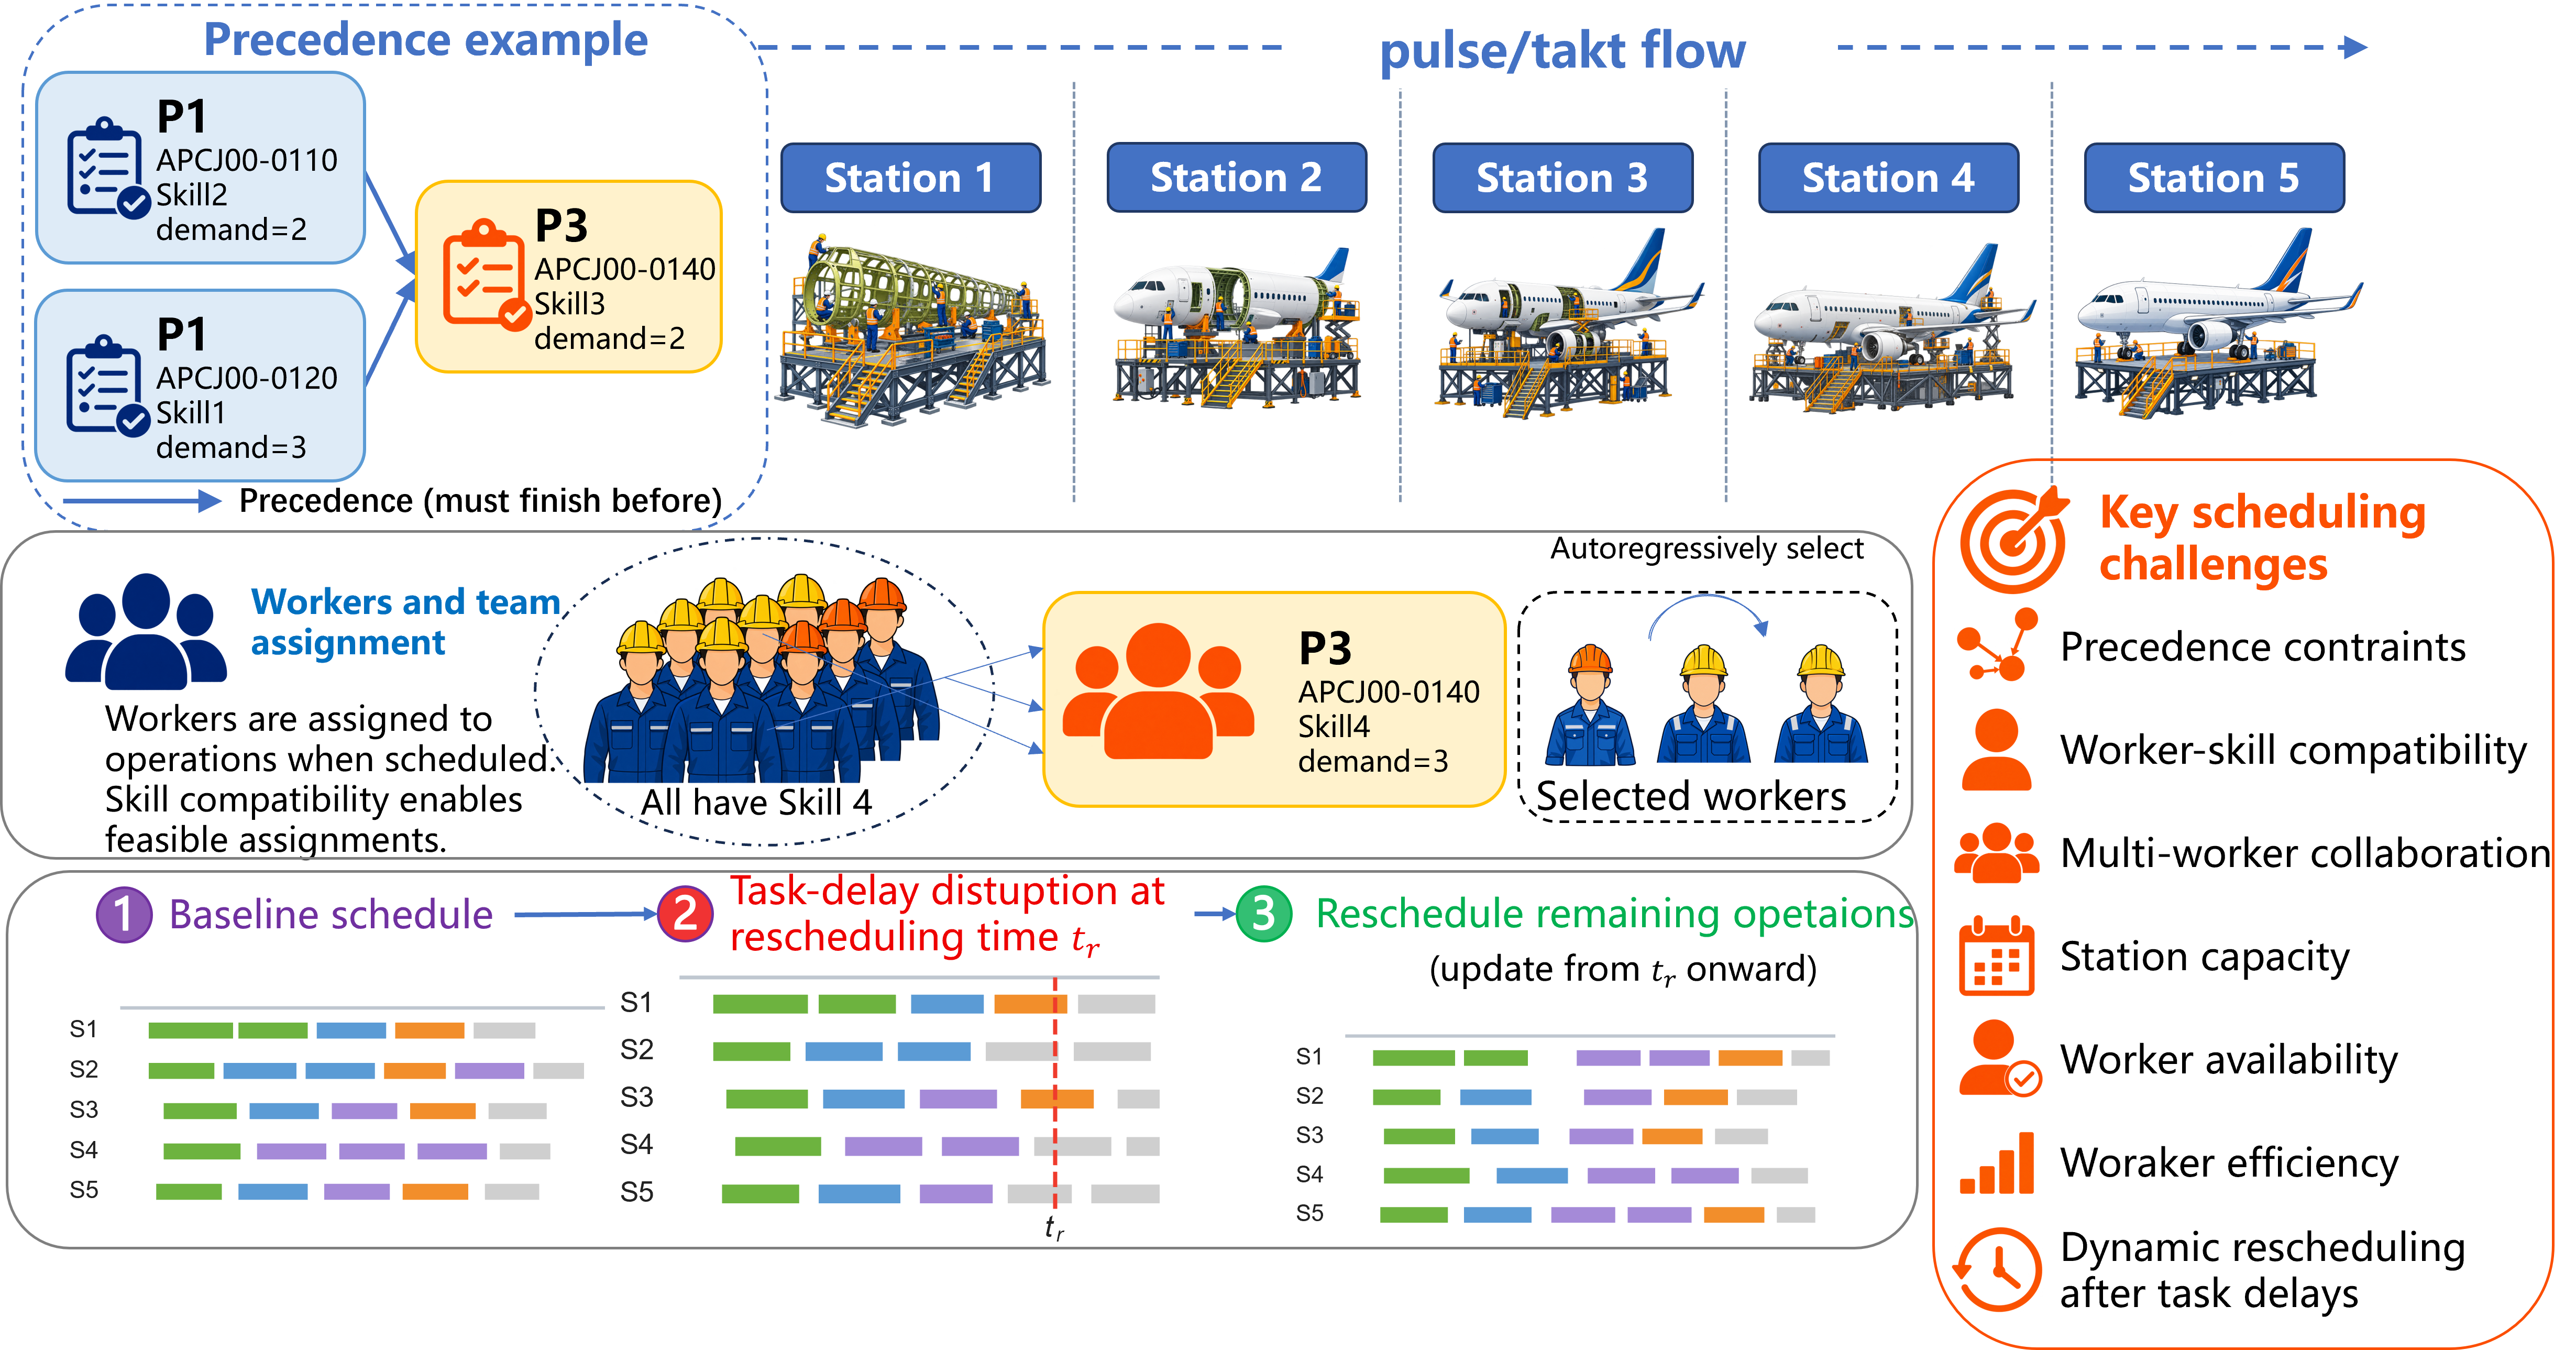
\includegraphics[width=0.92\textwidth,height=0.28\textheight,keepaspectratio]{figures/fig1.png}
\caption{Illustration of cyclic operation scheduling and stability-aware rescheduling for an aircraft pulsating assembly line. Aircraft advance through five physical stations in a pulsating rhythm. The cyclic operation template jointly determines the precedence-related execution relationships among operations, their assigned stations, and specific worker teams satisfying skill and headcount requirements. Following a material delay, the system locks committed entries at the schedule freeze boundary $\tau^r$, inherits worker bindings, and performs stability-aware rescheduling of the remaining operations.}
\label{fig:1}
\end{figure*}

This joint decision problem presents several challenges:
\begin{enumerate}
\item Operations, stations, workers, and skills exhibit heterogeneous multi-relational topologies, operating within an environment characterized by rapid state transitions and dynamic resource calendars;
\item Selecting an optimal team from a multiskilled labor pool results in a combinatorial team-selection space of size $\binom{n_i}{q_i}$ for each operation;
\item Each intermediate decision changes the feasible choices available to subsequent decisions;
\item When shop-floor disturbances such as material arrival delays occur, rescheduling must preserve frozen schedule entries and existing worker--station bindings while repairing subsequent cyclic templates to restore feasibility and balance completion span against deviations from the baseline schedule~\cite{vieira2003,hu2024}.
\end{enumerate}

Fig.~\ref{fig:1} illustrates the physical setting, entity interactions, and the plan repair process under material delay disturbances.

To address the coupling between operation scheduling and workforce allocation in aircraft pulsating assembly lines, this paper proposes the HGP-PPO joint scheduling framework. The main contributions are as follows:
\begin{enumerate}
\item \textbf{Joint scheduling model with endogenous workforce allocation:} An APAL cyclic operation template model is formulated to incorporate precedence constraints, station concurrency limits, and collaborative operations performed by multi-skilled workers. The model integrates operation-to-station assignment, selection of specific worker teams, and worker--station assignment into a unified sequential construction process. Persistent station bindings established upon each worker's first assignment explicitly capture how current team choices affect subsequent worker availability, enabling the coordinated determination of operation schedules and station workforce allocation.
\item \textbf{Heterogeneous graph representation of process dependencies and skill supply--demand relationships:} A heterogeneous graph comprising operation, station, worker, and skill nodes jointly represents process dependencies, skill supply--demand relationships, and dynamic assignments. Relation-specific attention encoding provides a shared state representation for operation-to-station assignment and team formation, enabling the policy to make joint decisions informed by both task structures and workforce states.
\item \textbf{Autoregressive joint decoding incorporating team states and skill scarcity:} A conditional operation--station--worker pointer mechanism decomposes the combinatorial selection of fixed-size teams into sequential member selections. Candidate workers are scored conditionally using partial team representations, tentative completion-time features, and the marginal scarcity of their additional skills. This mechanism avoids explicit enumeration of complete teams and uses dynamic masking and forward time allocation to enforce the scheduling constraints.
\end{enumerate}

The framework is evaluated for both initial scheduling and rescheduling under material readiness delays. For initial scheduling, a single policy is held fixed and applied without fine-tuning to four test instances containing 283 to 3,182 physical operations. Comparisons with workforce pre-assignment, alternative graph representations, and decision architectures assess the role of the overall design. The framework is then adapted to stability-oriented cyclic template rescheduling by incorporating baseline schedule and disturbance features and continuing training, while preserving frozen operations and existing worker--station bindings. Evaluation across 36 paired disturbance scenarios considers schedule feasibility, completion efficiency, deviations from the baseline schedule, and online solution time. Together, these experiments assess cross-scale applicability within the investigated APAL data family and the framework's applicability to both initial template construction and repair under material readiness delays.

The remainder of this paper is organized as follows: Section~\ref{sec:related} reviews related work. Section~\ref{sec:formulation} details the APAL scheduling and rescheduling models. Section~\ref{sec:method} presents the HGP-PPO methodology. Section~\ref{sec:experiments} provides experimental results and ablations. Section~\ref{sec:conclusions} concludes the paper with discussion on limitations and future avenues.

\section{Related Work}\label{sec:related}

\subsection{Aircraft Assembly Scheduling and Workforce Allocation}

Assembly line balancing and scheduling, spanning ALBP, SALBP, and GALBP, provide classical foundations for workload assignment across stations~\cite{becker2006,boysen2007,battaia2013}. In modern aerospace manufacturing, complex structural assembly operations have motivated the incorporation of multi-resource constraints. Bao \textit{et al.}~\cite{bao2023,bao2023b} addressed aircraft final assembly line balancing with resource constraints using staged heuristic searches. Fang \textit{et al.}~\cite{fang2021flexible} and Wang \textit{et al.}~\cite{wang2024} examined flexible cross-station workforce allocation. Liu \textit{et al.}~\cite{liu2025} and Wen \textit{et al.}~\cite{wen2026} studied multiskilled worker assignments and skill-grade matching during intra-station dispatching. While these studies underscore the decisive role of multi-resource allocation, most existing approaches treat station assignments as predetermined or restrict decision-making to aggregate workforce sizing. In contrast, this paper tackles a global setting where stations and worker teams are resolved jointly from globally unbound pools in a unified decision flow.

\subsection{Graph Reinforcement Learning for Production Scheduling}

Graph neural networks (GNNs) learn structural representations of combinatorial optimization problems through shared message-passing functions~\cite{cappart2023}. In job-shop (JSSP) and flexible job-shop scheduling (FJSP), graph-based reinforcement learning methods encode operation dependencies and machine constraints to learn dispatching policies~\cite{zhang2020,park2021,wang2024flexible}. In aerospace assembly, our preliminary work~\cite{ai2025} showed the promise of graph-enhanced reinforcement learning for pulsating lines. Wen \textit{et al.}~\cite{wen2026b} paired graph isomorphism networks (GIN) with PPO to address skill-level assembly scheduling. Nevertheless, standard RL action spaces typically focus on selecting a single operation or an operation--machine pair. To handle collaborative teams and dynamic station binding, the proposed framework represents process dependencies and skill supply--demand relationships through a heterogeneous graph and constructs teams using an operation--station--worker autoregressive decoder. Partial team states and skill-scarcity features inform successive member selections, while dynamic masks account for worker qualifications and station bindings.

\subsection{Assembly Line Rescheduling and Plan Stability}

In dynamic manufacturing, predictive--reactive scheduling provides a structured paradigm wherein baseline plans are formulated and subsequently revised upon disturbance arrivals~\cite{vieira2003,vonder2007}. Regarding supply chain disruptions, Zhu \textit{et al.}~\cite{zhu2021} adjusted unstarted operations for moving lines. Hu \textit{et al.}~\cite{hu2024} developed a two-stage robust strategy under processing-time variations, while Chen \textit{et al.}~\cite{chen2026} utilized multi-agent RL for dynamic dispatching under material delays. In APALs, rescheduling must account for synchronous line advancement. This study focuses on plan-level cyclic template rebalancing under material readiness delays, preserving frozen operations and existing worker--station bindings. Baseline schedule and disturbance features are incorporated into the joint decision framework, which is further trained to balance completion efficiency against deviations in operation start times, station assignments, and team composition.

\section{APAL Joint Scheduling and Rescheduling Problem Formulation}\label{sec:formulation}

\subsection{System Description, Assumptions, and Notation}

Consider an APAL comprising five fixed physical stations $\mathcal{M}=\{1,\dots,5\}$. The assembly process is represented by a directed acyclic graph (DAG) $G=(\mathcal{O},\mathcal{E})$, where $\mathcal{O}=\mathcal{O}^+\cup\mathcal{O}^0$. Here, $\mathcal{O}^+$ denotes physical operations with positive processing times, and $\mathcal{O}^0$ denotes non-executable process-structure nodes (having zero duration and retaining only process hierarchies, hereafter referred to as structural nodes). Structural nodes consume no physical resources. Physical precedence relations are derived by bypassing structural nodes while preserving the dependencies between physical operations, forming the physical operation DAG $G^+=(\mathcal{O}^+,\mathcal{E}^+)$. The immediate physical predecessors of operation $i$ are denoted by $\mathcal{P}(i)$.

The system includes a pool of multiskilled workers $\mathcal{W}$ and a set of five skill types $\mathcal{K}$. Each physical operation $i\in\mathcal{O}^+$ has a standard processing time $p_i^{\mathrm{std}}>0$, requires a single skill $k_i\in\mathcal{K}$, and demands a fixed collaborative team size $q_i\in\mathbb{N}^+$. Each worker $w\in\mathcal{W}$ has a binary skill qualification vector $\mathbf{H}_w=(H_{wk})_{k\in\mathcal{K}}$, where $H_{wk}\in\{0,1\}$, and a baseline efficiency coefficient $\eta_w>0$. Except for initial positioning tasks, operation stations are not predetermined.

The operational assumptions are established as follows:
\begin{enumerate}
\item \textbf{Non-preemptive execution}: Operations cannot be interrupted once initiated, and their allocated station and team cannot be altered.
\item \textbf{Worker binding upon first selection}: All workers are initially unbound ($\ell_w=\varnothing$). When worker $w$ is first assigned to an operation at station $m$, the worker is endogenously bound to station $m$ ($\ell_w=m$) for the entire scheduling episode and any subsequent rescheduling, preventing cross-station movement. Unbound workers remain globally available.
\item \textbf{Deterministic forward time allocation}: The policy generates discrete resource actions $(i, m_i, W_i)$ with $|W_i|=q_i$. The forward time allocation engine deterministically assigns the earliest feasible start time $B_i$ and finish time $C_i$ on the template timeline based on predecessor completions, worker calendars, material readiness, and station concurrency limits $c_m$.
\end{enumerate}

Table~\ref{tab:notation} outlines the mathematical notation used throughout this paper.

\begin{table}[!t]
\centering
\caption{Main Mathematical Notation}
\label{tab:notation}
\setlength{\tabcolsep}{3pt}
\renewcommand{\arraystretch}{1.05}
\begin{adjustbox}{max width=\columnwidth}
\begin{tabular}{@{}lp{6.8cm}@{}}
\toprule
\textbf{Symbol} & \textbf{Physical Meaning} \\
\midrule
$G^+=(\mathcal{O}^+,\mathcal{E}^+)$ & Physical operation DAG and its precedence edges \\
$\mathcal{M}, \mathcal{W}, \mathcal{K}$ & Physical stations ($|\mathcal{M}|=5$), worker pool, skill types ($|\mathcal{K}|=5$) \\
$p_i^{\mathrm{std}}, q_i, k_i$ & Standard duration, required team size, and skill type of operation $i$ \\
$H_{wk}, \eta_w$ & Binary skill indicator and baseline efficiency of worker $w$ \\
$c_m$ & Concurrency capacity (maximum simultaneous tasks) of station $m$ \\
$x_{im}, y_{iw}$ & Binary decision variables for station assignment and worker assignment \\
$m_i, W_i$ & Assigned physical station and specific team for operation $i$ ($|W_i|=q_i$) \\
$B_i, C_i$ & Start time and completion time of operation $i$ on template timeline \\
$\ell_w$ & Station binding of worker $w$; $\ell_w=\varnothing$ indicates an unbound worker \\
$\pi^0, T_{\mathrm{ref}}^0$ & Baseline template and reference cycle span $T_{\mathrm{ref}}^0:=H^0=C_{\max}(\pi^0)$ \\
$\tau^r, r_i$ & Rescheduling freeze boundary and updated material release time \\
$\mathcal{O}^{\mathrm{frz}}, \mathcal{O}^{\mathrm{mov}}$ & Frozen operations ($B_i^0\le\tau^r$) and reschedulable operations ($B_i^0>\tau^r$) \\
$H, C_{\max}, S$ & Cyclic template span, template makespan, and composite recovery objective \\
\bottomrule
\end{tabular}
\end{adjustbox}
\end{table}

\subsection{Initial APAL Cyclic Scheduling Model}

The processing duration of operation $i$ depends on the efficiencies of its assigned workers and a team coordination discount factor $\rho=0.95$:
\begin{equation}\label{eq:duration}
D_i(W_i) = \frac{p_i^{\mathrm{std}} q_i}{\rho^{q_i-1} \sum_{w\in W_i} \eta_w}.
\end{equation}

The optimization objective minimizes the template cycle span $H(\pi):=C_{\max}(\pi)$:
\begin{equation}\label{eq:cmax}
\min_{\pi}\; C_{\max}(\pi) = \max_{m\in\mathcal{M}} C_m^{\mathrm{end}}(\pi) = \max_{i\in\mathcal{O}^+} C_i,
\end{equation}
where $C_m^{\mathrm{end}}(\pi)=\max_{\{i\in\mathcal{O}^+\mid m_i=m\}} C_i$ represents the latest completion time at station $m$. Once the baseline schedule is fixed, its makespan defines the reference cycle span $T_{\mathrm{ref}}^0:=H^0=C_{\max}(\pi^0)$, which remains unchanged during rescheduling. Station labor load $L_m=\sum_{m_i=m} q_i D_i(W_i)$ serves as an intermediate diagnostic and reward-shaping signal.

The schedule must satisfy the following assignment, precedence, resource, and temporal constraints:
\begin{enumerate}
\item \textbf{Unique assignment and station monotonicity}:
\begin{equation}
\sum_{m\in\mathcal{M}} x_{im} = 1, \quad m_j \ge m_i, \quad \forall (i,j)\in\mathcal{E}^+.
\end{equation}
\item \textbf{Intra-template temporal precedence}:
\begin{equation}
B_j \ge C_i, \quad \forall (i,j)\in\mathcal{E}^+.
\end{equation}
\item \textbf{Team size, skill qualifications, and station exclusivity}:
\begin{equation}
\sum_{w\in\mathcal{W}} y_{iw} = q_i, \quad y_{iw} \le H_{w k_i}, \quad \forall i\in\mathcal{O}^+, w\in\mathcal{W};
\end{equation}
\begin{equation}
y_{iw} = y_{jw} = 1 \Longrightarrow m_i = m_j, \quad \forall i,j\in\mathcal{O}^+, w\in\mathcal{W}.
\end{equation}
\item \textbf{Temporal and spatial concurrency capacity}:
\begin{equation}
\sum_{i\in\mathcal{O}^+} y_{iw} \mathbb{I}(B_i \le t < C_i) \le 1, \quad \forall w\in\mathcal{W}, t\ge0;
\end{equation}
\begin{equation}
\sum_{i\in\mathcal{O}^+} x_{im} \mathbb{I}(B_i \le t < C_i) \le c_m, \quad \forall m\in\mathcal{M}, t\ge0.
\end{equation}
\item \textbf{Forward allocation lower bounds}:
\begin{equation}
B_i \ge \max\left\{c_t, \max_{j\in\mathcal{P}(i)} C_j, \max_{w\in W_i} a_w\right\},
\end{equation}
where $c_t$ is the current environment time clock and $a_w$ is the earliest available time of worker $w$.
\end{enumerate}

\subsection{Steady-State Cyclic Unfolding Across Aircraft}

\textbf{Proposition 1 (Physical feasibility of cyclic unfolding)}:
Given a feasible cyclic template $\pi = (m, W, B, C)$ satisfying all constraints in Section~\ref{sec:formulation}-B with span $H = C_{\max}$, let aircraft index be $k = 0, 1, 2, \dots$. For aircraft $k$, the execution interval of operation $i$ on the shop-floor timeline is
\begin{equation}
B_{i,k}^{\mathrm{phys}} = (k+m_i-1)H + B_i, \quad C_{i,k}^{\mathrm{phys}} = (k+m_i-1)H + C_i.
\end{equation}
Under these assumptions, the unfolded schedule preserves aircraft occupancy exclusivity, precedence feasibility, worker exclusivity, and station concurrency limits.

\textit{Proof}: Aircraft $k$ resides at station $m$ during $[(k+m-1)H, (k+m)H)$, and all its operations assigned to that station are contained within this window. Consecutive aircraft at the same station occupy non-overlapping intervals, ensuring spatial exclusivity. For any $(i,j)\in\mathcal{E}^+$, the physical time difference satisfies:
\begin{equation}
B_{j,k}^{\mathrm{phys}} - C_{i,k}^{\mathrm{phys}} = (m_j - m_i)H + (B_j - C_i) \ge 0.
\end{equation}
Since $m_j\ge m_i$ and $B_j\ge C_i$, physical precedence is naturally preserved. For cross-station dependencies where $m_j>m_i$, $(m_j-m_i)H\ge H$, meaning predecessor tasks were completed in earlier cycles. Imposing $B_j\ge C_i$ within a single template thus serves as a structured sufficient condition for physically executable multi-aircraft unfolding. \hfill $\blacksquare$

\subsection{Stability-Aware Template Rescheduling Under Material Delays}

When material for operation $i$ is delayed by $\Delta_i>0$, its release time updates to $r_i=B_i^0+\Delta_i$. At freeze boundary $\tau^r$, operations are partitioned into frozen set $\mathcal{O}^{\mathrm{frz}}=\{i\in\mathcal{O}^+\mid B_i^0\le\tau^r\}$ and reschedulable set $\mathcal{O}^{\mathrm{mov}}=\{i\in\mathcal{O}^+\mid B_i^0>\tau^r\}$.

\begin{enumerate}
\item \textbf{Frozen commitments}: Committed operations strictly inherit baseline assignments:
\begin{equation}
(m_i^r, W_i^r, B_i^r, C_i^r) = (m_i^0, W_i^0, B_i^0, C_i^0), \quad \forall i\in\mathcal{O}^{\mathrm{frz}}.
\end{equation}
\item \textbf{Worker binding inheritance}: Workers chosen in the baseline plan retain their station bindings ($\ell_w^r=m$). Only previously unused workers remain unbound.
\item \textbf{Reschedulable bounds}: Reschedulable operations must satisfy $B_i^r \ge \max\{\tau^r, r_i\}, \forall i\in\mathcal{O}^{\mathrm{mov}}$.
\end{enumerate}

Defining $N_{\mathrm{mov}}=|\mathcal{O}^{\mathrm{mov}}|$, baseline overrun $\Delta_{\mathrm{ref}}^r=\max\{0, C_{\max}^r-T_{\mathrm{ref}}^0\}$, start-time deviation $\bar D_{\mathrm{start}}^r=\frac{1}{N_{\mathrm{mov}}}\sum |B_i^r-B_i^0|$, station change rate $R_{\mathrm{sta}}^r=\frac{1}{N_{\mathrm{mov}}}\sum \mathbb{I}(m_i^r\ne m_i^0)$, and team change rate $R_{\mathrm{team}}^r=\frac{1}{N_{\mathrm{mov}}}\sum \mathbb{I}(W_i^r\ne W_i^0)$, the composite stability objective is formulated as:
\begin{equation}\label{eq:reschedule_obj}
\resizebox{0.88\linewidth}{!}{$\displaystyle
\min_{\pi^r\in\Pi_{\mathrm{feas}}^r}\; S(\pi^r) = 0.20\frac{C_{\max}^r}{T_{\mathrm{ref}}^0} + 3\frac{\Delta_{\mathrm{ref}}^r}{T_{\mathrm{ref}}^0} + 4\frac{\bar D_{\mathrm{start}}^r}{T_{\mathrm{ref}}^0} + 4 R_{\mathrm{sta}}^r + 0.3 R_{\mathrm{team}}^r.
$}
\end{equation}

\section{HGP-PPO Method}\label{sec:method}

\subsection{Unified Sequential MDP and Learning Framework}

Initial scheduling and stability-aware rescheduling are unified into a sequential MDP $\mathcal{M}^z=(\mathcal{S}^z,\mathcal{A},\mathcal{P},\mathcal{R}^z,\gamma), z\in\{\mathrm{init},\mathrm{res}\}$:
\begin{enumerate}
\item \textbf{State representation}: State $s_t$ at decision step $t$ is encoded as a four-entity heterogeneous graph $G_t$ capturing process dependencies, station loads, and worker availability calendars. The index $t$ denotes a scheduling decision step, whereas $c_t$ denotes the current environment time.
\item \textbf{Hierarchical action decomposition}: The discrete joint action $a_t=(i_t,m_t,W_t)$ ($|W_t|=q_{i_t}$) is autoregressively decomposed into an ordered trajectory $\widetilde a_t=(i_t,m_t,\mathbf w_t)$, mapped to unordered set $W_t$ upon team completion.
\item \textbf{Dynamic masking}: Hard constraints are enforced at each decision tier by masking invalid candidates with $-\infty$.
\item \textbf{Stage-specific rewards}: Initial scheduling uses differential makespan rewards and changes in the standard deviation of station labor loads: $\widetilde r_t^{\mathrm{init}} = -(\widehat C_{t+1}-\widehat C_t)/C_{\mathrm{ref}} - 0.5(\sigma_{L,t+1}-\sigma_{L,t})/L_{\mathrm{ref}}$; rescheduling directly adopts the negative composite score difference: $\widetilde r_t^{\mathrm{res}} = -[\widehat S(s_{t+1})-\widehat S(s_t)]$.
\end{enumerate}

Fig.~\ref{fig:2} presents the architectural layout of HGP-PPO.

\begin{figure*}[!t]
\centering
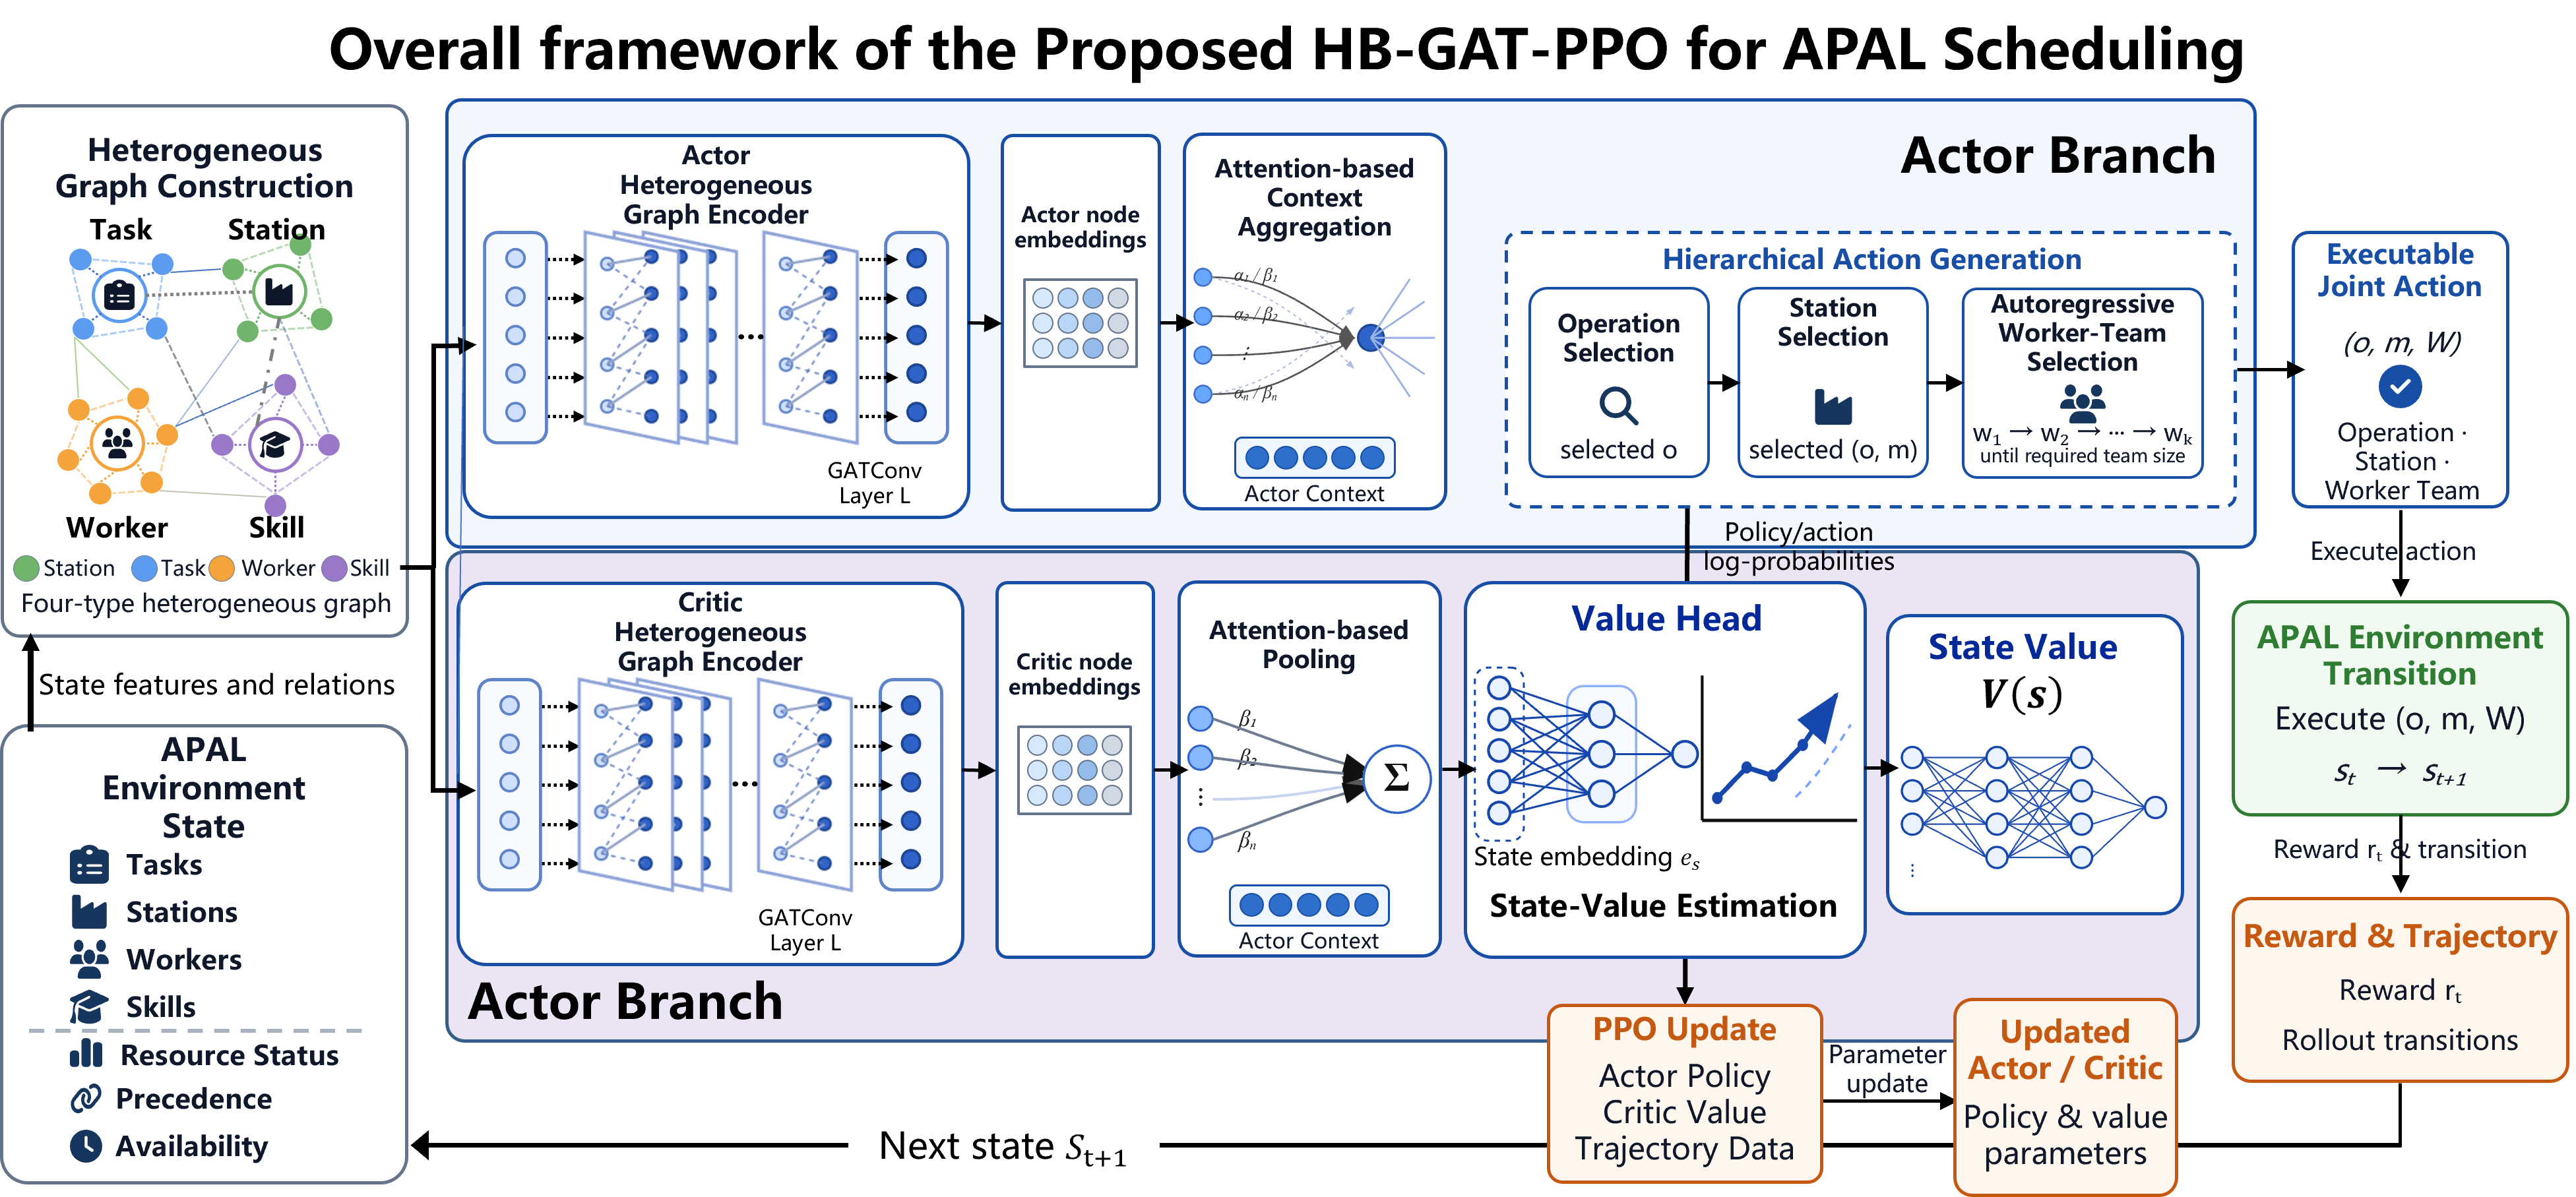
\includegraphics[width=0.92\textwidth,height=0.25\textheight,keepaspectratio]{figures/fig2.png}
\caption{Overall HGP-PPO framework. The APAL environment state is first converted into a heterogeneous graph with Operation, Station, Worker, and Skill nodes. The Actor and Critic use independent heterogeneous graph encoders. After attention-based context aggregation, the Actor sequentially selects an Operation, a Station, and a Worker team of the required size to form an executable joint action $(o,m,W)$. The Critic aggregates the graph state and estimates the state value $V(s)$. Executing the joint action produces the next state, reward, and trajectory, which PPO uses to update the policy and value networks.}
\label{fig:2}
\end{figure*}

\subsection{Heterogeneous Graph Representation and Global Encoding}\label{sec:encoder}

At decision step $t$, the state is represented by a heterogeneous graph $G_t=(\mathcal{V}_t,\mathcal{E}_t)$, where $\mathcal{V}_t=\mathcal{O}\cup\mathcal{M}\cup\mathcal{W}\cup\mathcal{K}$. The Operation node set $\mathcal{O}=\mathcal{O}^+\cup\mathcal{O}^0$ includes physical operations and auxiliary structural nodes retained from the source process graph. Structural nodes have zero duration and no physical resource requirements; they are retained for graph encoding but excluded from scheduling actions. Tables~\ref{tab:node_features} and~\ref{tab:relations} summarize the node features and relation types, respectively.

\begin{table}[!t]
\centering
\caption{Input State Features for the Four Node Types}
\label{tab:node_features}
\setlength{\tabcolsep}{3pt}
\renewcommand{\arraystretch}{1.05}
\begin{adjustbox}{max width=\columnwidth}
\begin{tabular}{@{}lp{6.8cm}@{}}
\toprule
\textbf{Node Type} & \textbf{State Features} \\
\midrule
Operation & Normalized duration $\widetilde p_i$, status, 5-dim skill requirement, team size $q_i$, release time; rescheduling adds baseline start, station, team size, and freeze/delay flags \\
Station & Cumulative labor load, bound/unbound worker ratios, slot waiting time, available concurrency slots \\
Worker & Baseline efficiency $\eta_w$, 5-dim skills, waiting time, idle flag, station binding $\ell_w$ \\
Skill & Category index, headcounts, available capacity, and mean efficiency of qualified workers \\
\bottomrule
\end{tabular}
\end{adjustbox}
\vspace{2pt}
\par\noindent{\scriptsize Note: Operation-specific resource requirements apply to physical operations.}\par
\end{table}

\begin{table}[!t]
\centering
\caption{Heterogeneous Graph Relations and Dynamics}
\label{tab:relations}
\setlength{\tabcolsep}{3pt}
\renewcommand{\arraystretch}{1.05}
\begin{adjustbox}{max width=\columnwidth}
\begin{tabular}{@{}llll@{}}
\toprule
\textbf{Relation} & \textbf{Edge Direction} & \textbf{Dynamics} & \textbf{Physical Meaning} \\
\midrule
precedes & Operation $\rightarrow$ Operation & Static & Process precedence dependency \\
assigned-to & Operation $\rightarrow$ Station & Dynamic & Task station assignment \\
has-task & Station $\rightarrow$ Operation & Dynamic & Station-hosted operations \\
done-by & Operation $\rightarrow$ Worker & Dynamic & Assigned team members \\
has-skill & Worker $\rightarrow$ Skill & Fixed & Worker skill qualification \\
provided-by & Skill $\rightarrow$ Worker & Fixed & Skill-holding workforce \\
requires & Operation $\rightarrow$ Skill & Static & Operation skill requirement \\
required-by & Skill $\rightarrow$ Operation & Static & Operations requiring skill \\
\bottomrule
\end{tabular}
\end{adjustbox}
\end{table}

Skill nodes bridge operation skill requirements with worker skill competencies, enabling operations sharing identical skill demands and workers possessing multiple qualifications to engage in message passing through explicit relational edges. In conjunction with process precedence and dynamic assignment relations, this representation establishes a unified graph context for the policy to evaluate immediate task demands and concurrent labor competition. Raw features are projected into a $d$-dimensional space $\mathbf h_v^{(0)}=f_X(\mathbf x_v)$. Message passing is executed across $L=5$ relation-specific GATv2 layers~\cite{brody2022}. For edge $u\rightarrow v$ under relation $r$, head $h$:
\begin{center}
\begin{adjustbox}{max width=\linewidth}
$\displaystyle
e_{uv}^{(r,\ell,h)} = \mathbf a_{r,h}^{(\ell)\top}\operatorname{LeakyReLU}\left(\mathbf W_{s,r,h}^{(\ell)}\mathbf h_u^{(\ell-1)} + \mathbf W_{t,r,h}^{(\ell)}\mathbf h_v^{(\ell-1)}\right), \quad
\alpha_{uv}^{(r,\ell,h)} = \frac{\exp\left(e_{uv}^{(r,\ell,h)}\right)}{\sum_{z\in\mathcal N_r(v)}\exp\left(e_{zv}^{(r,\ell,h)}\right)}.
$
\end{adjustbox}
\end{center}
Aggregating multi-head messages $\mathbf m_v^{(r,\ell)} = \frac{1}{H}\sum_{h=1}^H\sum_{u\in\mathcal N_r(v)}\alpha_{uv}^{(r,\ell,h)}\mathbf W_{s,r,h}^{(\ell)}\mathbf h_u^{(\ell-1)}$:
\begin{equation}
\mathbf h_v^{(\ell)} = \mathbf h_v^{(\ell-1)} + \operatorname{LeakyReLU}\left(\sum_{r\in\mathcal R_{\mathrm{in}}(v)}\mathbf m_v^{(r,\ell)}\right).
\end{equation}

Node-type attention pooling produces a fixed-dimensional, permutation-invariant global context $\mathbf g_t=[\mathbf g_M \,\|\, \mathbf g_O \,\|\, \mathbf g_W]\in\mathbb R^{3d}$:
\begin{equation}
\beta_v^X = \frac{\exp(a_X(\mathbf h_v))}{\sum_{u\in\mathcal V^X}\exp(a_X(\mathbf h_u))}, \quad \mathbf g_X = \sum_{v\in\mathcal V^X}\beta_v^X\mathbf h_v.
\end{equation}

\subsection{Hierarchical Autoregressive Joint Decoding}

\textbf{Action probability factorization}:
Let $\mathbf w_t=(w_t^{(1)},\dots,w_t^{(q_{i_t})})$ denote the ordered worker generation trajectory and $W_t=\{w_t^{(1)},\dots,w_t^{(q_{i_t})}\}$ the resulting team. With trajectory action $\widetilde a_t=(i_t,m_t,\mathbf w_t)$ and execution action $a_t=(i_t,m_t,W_t)$:
\begin{center}
\begin{adjustbox}{max width=\linewidth}
$\displaystyle
\pi_\theta(\widetilde a_t\mid s_t) = \pi_O(i_t\mid s_t)\,\pi_M(m_t\mid s_t,i_t)\prod_{r=1}^{q_{i_t}}\pi_W\left(w_t^{(r)}\mid s_t,i_t,m_t,\mathbf w_t^{(<r)}\right).
$
\end{adjustbox}
\end{center}
PPO computes likelihoods on the ordered trajectory $\widetilde a_t$, while environment dynamics execute unordered set $W_t$.

\textbf{Operation and station pointers}:
The operation pointer selects from $\mathcal{F}_t^O\subseteq\mathcal{O}^+$, while the station pointer conditions on $\mathbf{h}_{i_t}$ over $\mathcal{F}_{i_t,t}^M$:
\begin{center}
\begin{adjustbox}{max width=\linewidth}
$\displaystyle
u_{i,t}^O = \mathbf a_O^{\top}\tanh(\mathbf W_g\mathbf g_t + \mathbf W_O\mathbf h_i), \qquad \pi_O(i\mid s_t) = \frac{\exp(u_{i,t}^O)}{\sum_{j\in\mathcal F_t^O}\exp(u_{j,t}^O)};
$
\end{adjustbox}
\end{center}
\begin{center}
\begin{adjustbox}{max width=\linewidth}
$\displaystyle
u_{m,t}^M = \mathbf a_M^{\top}\tanh(\mathbf W_{OM}\mathbf h_{i_t} + \mathbf W_M\mathbf h_m), \qquad \pi_M(m\mid s_t,i_t) = \frac{\exp(u_{m,t}^M)}{\sum_{n\in\mathcal F_{i_t,t}^M}\exp(u_{n,t}^M)}.
$
\end{adjustbox}
\end{center}
For worker selection, Worker Pointer scores candidates at substep $r\in\{1,\dots,q_{i_t}\}$:
\begin{center}
\begin{adjustbox}{max width=\linewidth}
$\displaystyle
u_{w,t}^{(r)} = \mathbf v_W^{\top}\tanh\left(\mathbf q_t^{(r)} + \mathbf k_{w,t}^{(r)}\right), \quad
\pi_W\left(w\mid s_t,i_t,m_t,\mathbf w_t^{(<r)}\right) = \frac{\exp(u_{w,t}^{(r)})}{\sum_{v\in\mathcal F_{W,t}^{(r)}}\exp(u_{v,t}^{(r)})}.
$
\end{adjustbox}
\end{center}
Infeasible candidates receive zero probability. Query $\mathbf q_t^{(r)}$ and key $\mathbf k_{w,t}^{(r)}$ incorporate skill pressures, dynamic EFT, and marginal scarcity (detailed in Appendix~\ref{app:worker_pointer}).

\textbf{Endogenous binding}:
\begin{equation}
\ell_{w,t+1} = \begin{cases} m_t, & \ell_{w,t}=\varnothing \ \text{and}\ w\in W_t, \\ \ell_{w,t}, & \text{otherwise}. \end{cases}
\end{equation}

\subsection{PPO Learning and Transfer}

With continuation indicator $b_t=(1-d_t)(1-u_t)$, temporal-difference error $\delta_t$ and GAE $\widehat A_t$ are:
\begin{equation}
\delta_t = r_t + \gamma b_t V_{\phi^-}(s_{t+1}) - V_{\phi^-}(s_t), \quad \widehat A_t = \delta_t + \gamma\lambda b_t \widehat A_{t+1}.
\end{equation}
Clipped PPO loss with ratio $r_t^{\mathrm{PPO}}(\theta)=\exp(\ell_{t,\theta}-\ell_{t,\theta^-})$ is:
\begin{equation}
\resizebox{0.95\linewidth}{!}{$\displaystyle
\mathcal L_{\mathrm{policy}}(\theta) = -\mathbb E_t\left[\min\left(r_t^{\mathrm{PPO}}(\theta)\widetilde A_t,\, \operatorname{clip}(r_t^{\mathrm{PPO}}(\theta), 1-\epsilon, 1+\epsilon)\widetilde A_t\right)\right],
$}
\end{equation}
\begin{equation}
\mathcal L = \mathcal L_{\mathrm{policy}}(\theta) + c_V \mathbb E_t[(V_\phi(s_t)-R_t)^2] - c_H \overline H.
\end{equation}
Shared graph-encoding and pointer parameters accommodate varying numbers of operations and workers without size-specific output heads, with scale-extrapolated schedule quality verified experimentally in Section~\ref{sec:experiments}. For rescheduling, operation node features expand from 18 to 24 dimensions to incorporate baseline schedules and disturbance signals, widening the first-layer operation projection matrix. Compatible parameters across the graph encoder, pooling layers, and pointer decoders are directly initialized from the trained initial-scheduling model; for the operation projection layer, weights corresponding to existing channels are preserved while new input channels are initialized under standard initialization. The policy is then further trained in the disturbance environment under the composite stability objective $S(\pi^r)$ with inherited worker--station bindings, enabling effective knowledge transfer from baseline scheduling to disturbance recovery.

\section{Experiments and Results}\label{sec:experiments}

\subsection{Evaluation Questions and Protocol}

Experiments investigate five core evaluation questions:
\begin{itemize}
\item \textbf{EQ1 (Scale extrapolation)}: Can a locked policy generalize to 283--3,182 physical operations without fine-tuning?
\item \textbf{EQ2 (Decoding quality)}: Does autoregressive joint decoding outperform heuristics and RL baselines in makespan $H=C_{\max}$?
\item \textbf{EQ3 (Structural ablations)}: Do heterogeneous graph attention, endogenous binding, and three-tier decisions match APAL physics?
\item \textbf{EQ4 (Online runtime)}: How does neural forward inference scale against per-instance search algorithms?
\item \textbf{EQ5 (Disturbance recovery)}: Can the architecture balance feasibility, makespan, and stability under material delays?
\end{itemize}

\textbf{Dataset partitioning}:
\begin{itemize}
\item \textbf{Training}: 24 synthetic variants (400--800 operations) for gradient optimization;
\item \textbf{Development}: 6 instances and 54 delay scenarios for hyperparameter selection and early stopping;
\item \textbf{Locked test}: 4 real factory instances (Table~\ref{tab:instances}) and 36 fixed disturbance scenarios evaluated once without post-hoc tuning.
\end{itemize}
Completeness ($R_{\mathrm{complete}}=1$) and physical validity ($R_{\mathrm{valid}}=1$) are strict prerequisites for quality ranking. Physical precedence relations are derived by bypassing structural nodes while preserving the dependencies between physical operations.

\begin{table}[!t]
\centering
\caption{Real Factory APAL Locked Evaluation Instances}
\label{tab:instances}
\setlength{\tabcolsep}{6pt}
\renewcommand{\arraystretch}{1.05}
\begin{adjustbox}{max width=\columnwidth}
\begin{tabular}{@{}cccc@{}}
\toprule
\textbf{Instance} & \textbf{Physical operations} & \textbf{Stations} & \textbf{Role} \\
\midrule
283 & 283 & 5 & Locked test \\
680 & 680 & 5 & Locked test \\
2338 & 2,338 & 5 & Locked test \\
3182 & 3,182 & 5 & Locked test \\
\bottomrule
\end{tabular}
\end{adjustbox}
\vspace{2pt}
\par\noindent{\scriptsize Note: Instance sizes count physical operations only. Source process graphs additionally contain 7, 35, 64, and 117 structural nodes (290, 715, 2,402, and 3,299 total nodes).}\par
\end{table}

\begin{table}[!t]
\centering
\caption{Comparison Methods, Decision Logic, and Search Budgets}
\label{tab:baselines}
\setlength{\tabcolsep}{3pt}
\renewcommand{\arraystretch}{1.05}
\begin{adjustbox}{max width=\columnwidth}
\begin{tabular}{@{}lll@{}}
\toprule
\textbf{Category} & \textbf{Method} & \textbf{Decision Criteria / Search Budget} \\
\midrule
Dispatching rules & SPT~\cite{smith1956} / LPT & Shortest / longest standard duration first \\
Dispatching rules & ES / CPM~\cite{kelley1961} / MSL & Earliest start / critical-path start / min slack \\
Dispatching rules & Random & Fixed seed random selection \\
Metaheuristics & Beam Search~\cite{ow1988} & Priorities search; init: $w=4, b=4$; resched: $w=2, b=2$ \\
Metaheuristics & IG~\cite{ruiz2007} & Iterated greedy; init: 160 iters; resched: 3 iters \\
Metaheuristics & SA~\cite{kirkpatrick1983} & Simulated annealing; init: 120 iters; resched: 3 iters \\
RL baselines & L2D-PPO-APAL & Graph dispatching policy adapted to APAL \\
RL baselines & Graph-DDQN-APAL & Graph value-based RL adapted to APAL \\
Reference & NoReschedule & Negative control: retain unadjusted baseline \\
Heuristic repair & StabilityAware / CPM & Multi-objective hybrid priority repair \\
\bottomrule
\end{tabular}
\end{adjustbox}
\end{table}

\subsection{Comparison Methods and Statistical Inference}

Table~\ref{tab:baselines} outlines the comparison methods. Initial scheduling is evaluated on deterministic makespan $H=C_{\max}$ (Eq.~\eqref{eq:cmax}), supplemented by five random seeds. Rescheduling is evaluated via composite score $S$ (Eq.~\eqref{eq:reschedule_obj}) across 36 paired disturbance scenarios. Overall significance is assessed via Friedman test across 19 feasible methods ($\chi_F^2(18)=369.20, p<0.001$), paired two-sided Wilcoxon signed-rank tests with Holm--Bonferroni correction, and 10,000 stratified bootstrap resamples for 95\% confidence intervals.

\begin{table*}[!t]
\centering
\caption{Initial Scheduling Makespan Across Four APAL Instances (h; Lower Is Better)}
\label{tab:initial_results}
\setlength{\tabcolsep}{8pt}
\renewcommand{\arraystretch}{1.06}
\begin{adjustbox}{max width=\textwidth}
\begin{tabular}{@{}llrrrrr@{}}
\toprule
\textbf{Category} & \textbf{Method} & \textbf{283} & \textbf{680} & \textbf{2338} & \textbf{3182} & \textbf{Mean Across Scales} \\
\midrule
Graph RL & \textbf{Proposed HGP-PPO} & 286.96 & \textbf{489.00} & 1209.96 & \textbf{1623.69} & \textbf{902.40} \\
Allocation ablation & Worker--Station Preassignment & 320.31 & 959.63 & 1605.13 & 2645.84 & 1382.73 \\
RL baselines & L2D-PPO-APAL & 288.97 & 518.65 & \textbf{1079.44} & 1804.71 & 922.94 \\
RL baselines & Graph-DDQN-APAL & \textbf{286.77} & 612.29 & 1263.66 & 2049.70 & 1053.11 \\
Metaheuristics & Iterated Greedy (IG) & 339.05 & 961.10 & 1797.57 & 2759.01 & 1464.18 \\
Metaheuristics & Beam Search & 333.43 & 984.30 & 1904.88 & 3272.54 & 1623.79 \\
Metaheuristics & Simulated Annealing (SA) & 311.78 & 1238.00 & 2417.03 & 3256.29 & 1805.77 \\
Dispatching rules & LPT & 292.63 & 637.56 & 1497.35 & 2039.50 & 1116.76 \\
Dispatching rules & Random & 310.62 & 872.52 & 1414.20 & 2170.15 & 1191.87 \\
Dispatching rules & SPT & 411.57 & 1702.77 & 2479.07 & 3346.37 & 1984.94 \\
Dispatching rules & MSL & 412.56 & 1608.50 & 2496.05 & 3455.45 & 1993.14 \\
Dispatching rules & ES-priority & 435.13 & 1773.41 & 2780.24 & 3729.75 & 2179.63 \\
Dispatching rules & CPM & 387.28 & 1597.92 & 2522.96 & 3430.06 & 1984.55 \\
\bottomrule
\end{tabular}
\end{adjustbox}
\par\smallskip
{\footnotesize Note: Deterministic masked argmax decoding. All methods share identical forward allocation and physical constraints.}
\end{table*}

\subsection{Initial Scheduling Results Across Scales}

Table~\ref{tab:initial_results} reports initial makespans. Across the four scales, HGP-PPO achieves the lowest equal-weight average makespan of 902.40~h, outperforming L2D-PPO-APAL (922.94~h) by 2.22\% and Graph-DDQN-APAL (1053.11~h) by 14.31\%. On the largest 3,182-operation instance, HGP-PPO achieves 1,623.69~h, reducing makespan by 181.02~h (10.03\%) compared to L2D-PPO-APAL. Metaheuristics (1464.18--1805.77~h) and dispatching rules (1116.76--2179.63~h) degrade noticeably at larger scales under the prespecified search budgets. Supplementary stochastic evaluations yield $274.97\pm3.77$, $517.50\pm12.89$, $1070.71\pm101.12$, and $1678.47\pm55.94$~h, averaging 885.41~h.

\begin{figure}[!t]
\centering
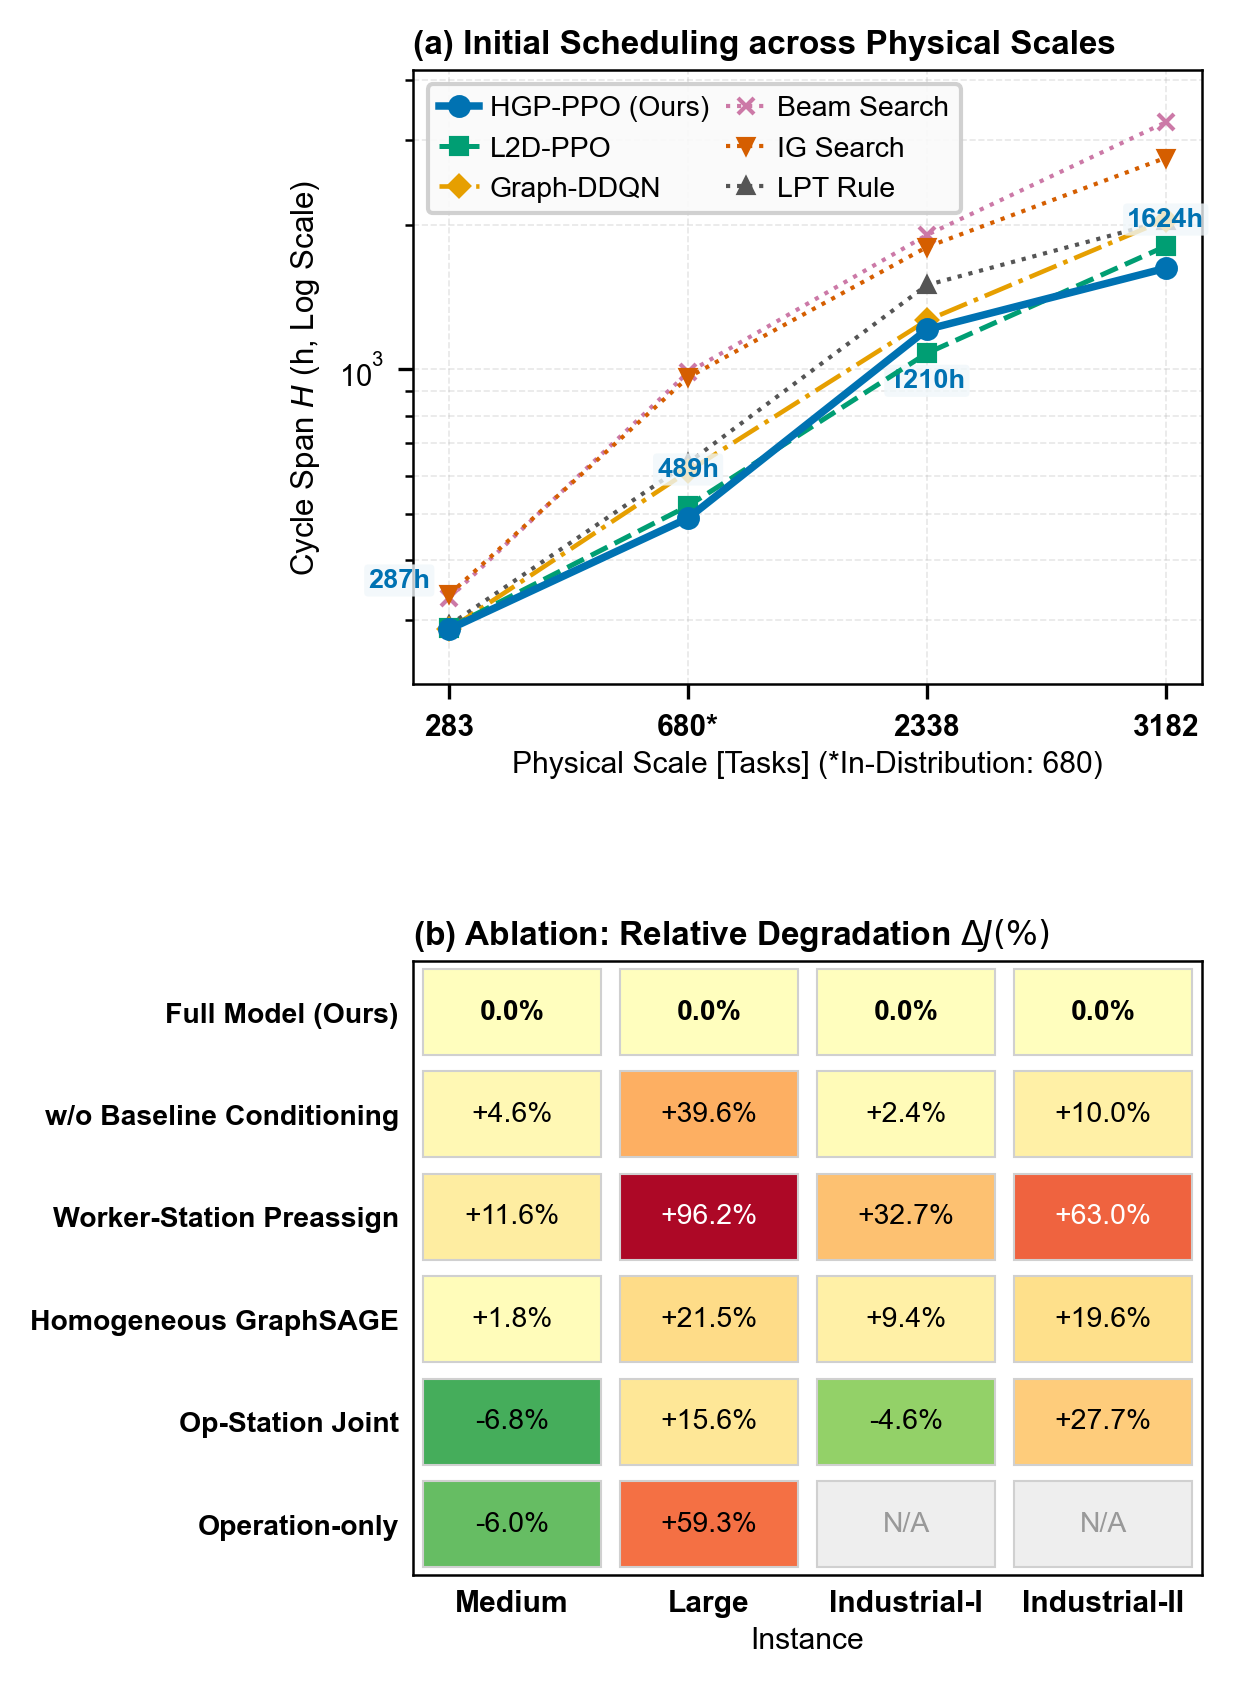
\includegraphics[width=\columnwidth]{figures/fig3_initial_and_ablation.png}
\caption{Initial scheduling performance across physical scales and architectural ablations. (a) Cycle spans $H$ on logarithmic axis across scales. (b) Relative degradation matrix $\Delta J(\%)$ against the full HGP-PPO architecture.}
\label{fig:3}
\end{figure}

\begin{table*}[!t]
\centering
\caption{Initial Makespans and Rescheduling Feasibility for Structural Variants}
\label{tab:ablation}
\setlength{\tabcolsep}{6pt}
\renewcommand{\arraystretch}{1.06}
\begin{adjustbox}{max width=\textwidth}
\begin{tabular}{@{}llrrrrrcc@{}}
\toprule
\textbf{Method} & \textbf{Structural Modification} & \textbf{283} & \textbf{680} & \textbf{2338} & \textbf{3182} & \textbf{Mean} & \textbf{Init Feas.} & \textbf{Resched Feas.} \\
\midrule
\textbf{Proposed HGP-PPO} & Full heterogeneous graph; joint Op--St--Wk decisions & 286.96 & 489.00 & 1209.96 & 1623.69 & \textbf{902.40} & 4/4 & \textbf{100\%} \\
Homogeneous GraphSAGE & Homogeneous graph encoding without typed message passing & 292.02 & 594.04 & 1323.22 & 1941.29 & 1037.64 & 4/4 & 100\% \\
Op--Station Decisions & Rule-based worker selection without explicit worker pointer & \textbf{267.40} & 565.26 & \textbf{1154.20} & 2073.34 & 1015.05 & 4/4 & \phantom{00}0\% \\
Op-Only Decisions & Heuristic station and worker dispatching & 269.66 & 779.13 & Infeas. & Infeas. & --- & 2/4 & 100\% \\
\bottomrule
\end{tabular}
\end{adjustbox}
\par\smallskip
{\footnotesize Note: Feasibility rates computed across 36 paired disturbance scenarios. Infeasible instances are excluded from mean makespan calculations.}
\end{table*}

\subsection{Decision Architecture and Configuration Comparisons}

Table~\ref{tab:ablation} and Fig.~\ref{fig:3} analyze structural ablations:
\begin{enumerate}
\item \textbf{Worker--Station preassignment}: Pre-fixing worker--station assignments inflates average makespan to 1,382.73~h (+53.2\%), indicating that static allocation bottlenecks task execution.
\item \textbf{Homogeneous GraphSAGE}: Collapsing heterogeneous relations increases mean makespan to 1,037.64~h (+15.0\%).
\item \textbf{Op--Station decisions}: Bypassing worker pointers yields low initial makespans on smaller instances but leads to a 0\% feasibility rate during rescheduling due to team allocation deadlocks.
\item \textbf{Op-only decisions}: Omitting station pointers results in infeasibility on instances with 2,338 and 3,182 operations.
\end{enumerate}

\begin{table*}[!t]
\centering
\caption{Composite Scores and Mean Makespans for Rescheduling Across 36 Material Delay Scenarios}
\label{tab:resched_master}
\setlength{\tabcolsep}{6pt}
\renewcommand{\arraystretch}{1.06}
\begin{adjustbox}{max width=\textwidth}
\begin{tabular}{@{}llrrrrrcc@{}}
\toprule
\textbf{Category} & \textbf{Method} & \textbf{283} & \textbf{680} & \textbf{2338} & \textbf{3182} & \textbf{Mean $S$} & \textbf{Makespan (h)} & \textbf{Feasibility} \\
\midrule
Graph RL & \textbf{Proposed HGP-PPO} & 0.9572 / 297.7 & 0.7621 / 674.9 & 0.8627 / 1223.9 & 0.8224 / 1709.5 & \textbf{0.8511} & 976.5 & \textbf{100\%} \\
Model variant & Ablated model without baseline conditioning & 0.9700 / 300.1 & 0.8242 / 682.5 & 0.9186 / 1239.2 & 1.0588 / 1786.6 & 0.9429 & 1002.1 & 100\% \\
Ablation & Homogeneous GraphSAGE & 1.2236 / 318.9 & 1.0447 / 682.4 & 1.0310 / 1263.2 & 1.1599 / 1806.8 & 1.1148 & 1017.8 & 100\% \\
Ablation & Operation-only decisions & 0.9592 / 296.9 & 1.2479 / 678.6 & 1.0825 / 1223.8 & 1.6577 / 1903.3 & 1.2368 & 1025.7 & 100\% \\
RL baselines & L2D-PPO-APAL & 0.9439 / 301.3 & 0.8441 / 663.3 & 0.8401 / 1223.9 & 1.0325 / 1764.9 & 0.9152 & 988.3 & 100\% \\
RL baselines & Graph-DDQN-APAL & 1.0414 / 306.6 & 1.0714 / 672.8 & 0.9394 / 1223.9 & 0.8716 / 1709.9 & 0.9810 & 978.3 & 100\% \\
Metaheuristics & BeamSearchRepair & 1.0575 / 322.9 & 1.0763 / 752.4 & 1.2596 / 1403.6 & 1.3626 / 1987.2 & 1.1890 & 1116.5 & 100\% \\
Metaheuristics & IteratedGreedyRepair & 1.0312 / 319.1 & 1.6770 / 783.1 & 1.6892 / 1454.1 & 1.3655 / 1987.5 & 1.4407 & 1135.9 & 100\% \\
Metaheuristics & SimulatedAnnealingRepair & 1.1431 / 323.6 & 2.2088 / 814.1 & 1.8923 / 1484.4 & 1.4394 / 2001.8 & 1.6709 & 1156.0 & 100\% \\
Heuristic repair & HybridCPMStabilityRepair & 1.1337 / 294.2 & 1.0463 / 675.4 & 0.9952 / 1223.9 & 0.7560 / 1665.9 & 0.9828 & \textbf{964.9} & 100\% \\
Heuristic repair & StabilityAwareRepair & 0.9913 / 310.4 & 0.7554 / 682.7 & 0.8045 / 1229.4 & 0.9591 / 1752.8 & 0.8776 & 993.8 & 100\% \\
Heuristic repair & TaktAwareRepair & 0.9103 / 323.8 & 1.0759 / 775.7 & 1.0398 / 1307.4 & 0.9073 / 1816.4 & 0.9833 & 1055.8 & 100\% \\
Heuristic repair & ReleaseAwareRepair & 0.7844 / 316.8 & 1.4584 / 770.5 & 1.1644 / 1369.4 & 1.1556 / 1901.5 & 1.1407 & 1089.5 & 100\% \\
Heuristic repair & BottleneckSkillRepair & 0.9667 / 326.4 & 1.4732 / 768.0 & 1.4282 / 1404.7 & 0.8398 / 1827.5 & 1.1770 & 1081.7 & 100\% \\
Heuristic repair & SPTRepair & 1.0188 / 333.3 & 0.9794 / 758.4 & 1.1850 / 1373.5 & 1.2038 / 1914.2 & 1.0967 & 1094.9 & 100\% \\
Heuristic repair & FullRescheduleCPM & 1.3579 / 332.0 & 1.5415 / 778.9 & 1.5528 / 1384.3 & 1.1864 / 1875.6 & 1.4097 & 1092.7 & 100\% \\
Heuristic repair & CPMRepair & 1.3513 / 331.1 & 1.5147 / 773.9 & 1.5968 / 1396.1 & 1.1838 / 1880.2 & 1.4116 & 1095.3 & 100\% \\
Heuristic repair & LPTRepair & 1.5492 / 345.0 & 2.6828 / 836.3 & 1.9494 / 1456.0 & 1.3546 / 1922.1 & 1.8840 & 1139.9 & 100\% \\
Heuristic repair & RandomRepair & 1.5427 / 351.7 & 3.2131 / 943.2 & 2.6982 / 1673.2 & 1.9854 / 2153.4 & 2.3599 & 1280.4 & 100\% \\
Negative control & NoReschedule & --- & --- & --- & --- & N/A & N/A & \phantom{00}0\% \\
\bottomrule
\end{tabular}
\end{adjustbox}
\par\smallskip
{\footnotesize Note: Entries formatted as ``$S$ / makespan (h)''. Scores normalized by $T_{\mathrm{ref}}^0$ and averaged equally across scenarios and instances.}
\end{table*}

\begin{table}[!t]
\centering
\caption{Raw Rescheduling Physical Component Decomposition}
\label{tab:raw_components}
\setlength{\tabcolsep}{3pt}
\renewcommand{\arraystretch}{1.05}
\begin{adjustbox}{max width=\columnwidth}
\begin{tabular}{@{}lrrrrrr@{}}
\toprule
\textbf{Method} & $C_{\max}$~(h) & $\Delta_{\mathrm{ref}}$~(h) & $\bar D_{\mathrm{start}}$~(h) & $R_{\mathrm{sta}}$~(\%) & $R_{\mathrm{team}}$~(\%) & \textbf{Score} $S$ \\
\midrule
\textbf{Proposed} & 976.49 & 29.51 & \textbf{30.85} & 2.12 & 95.60 & \textbf{0.851100} \\
L2D-PPO & 988.33 & 42.11 & 45.54 & 1.93 & 95.87 & 0.915151 \\
Graph-DDQN & 978.32 & 29.63 & 56.31 & 2.02 & 96.05 & 0.980965 \\
BeamSearch & 1116.52 & 167.19 & 108.85 & \textbf{0.54} & \textbf{0.70} & 1.188985 \\
HybridCPM & \textbf{964.87} & \textbf{18.79} & 61.76 & 1.85 & 93.53 & 0.982793 \\
StabilityAware & 993.85 & 45.22 & 33.88 & 1.73 & 94.76 & 0.877564 \\
\bottomrule
\end{tabular}
\end{adjustbox}
\par\smallskip
{\footnotesize Note: $R_{\mathrm{team}}$ is evaluated on reschedulable tasks: replacing any member counts as a team modification without implying cross-station mobility.}
\end{table}

\begin{table*}[!t]
\centering
\caption{Paired Rescheduling Statistics Against the Two Closest Baselines}
\label{tab:paired_stats}
\setlength{\tabcolsep}{8pt}
\renewcommand{\arraystretch}{1.06}
\begin{adjustbox}{max width=\textwidth}
\begin{tabular}{@{}lcccccc@{}}
\toprule
\textbf{Baseline Method} & \textbf{Mean $S$ Difference} & \textbf{Relative Reduction} & \textbf{Wins / Ties / Losses} & $p_{\mathrm{Holm}}$ & $r_{\mathrm{rb}}$ & \textbf{Stratified Bootstrap 95\% CI} \\
\midrule
L2D-PPO-APAL & $-0.0640$ & 7.00\% & 19 / 0 / 17 & 0.7237 & $-0.069$ & $[-0.1344, -0.0023]$ \\
StabilityAwareRepair & $-0.0265$ & 3.01\% & 22 / 0 / 14 & 0.5498 & $-0.210$ & $[-0.0652, \phantom{-}0.0110]$ \\
\bottomrule
\end{tabular}
\end{adjustbox}
\par\smallskip
{\footnotesize Note: Negative differences indicate proposed method superiority. $p_{\mathrm{Holm}}$ denotes two-sided Wilcoxon corrected across 18 baselines; CI based on 10,000 resamples.}
\end{table*}
\newpage
\subsection{Rescheduling Results Under Material Delays}

Table~\ref{tab:resched_master} summarizes results across 36 scenarios. HGP-PPO achieves the lowest average composite score of $S=0.8511$, outperforming StabilityAwareRepair (0.8776), L2D-PPO-APAL (0.9152), and Graph-DDQN-APAL (0.9810). Its median and IQM scores are 0.7415 and 0.7670, with the lowest ARD of 26.60\% and the lowest average rank (4.56).

Table~\ref{tab:raw_components} decomposes the physical components. Compared with StabilityAwareRepair, HGP-PPO reduces average makespan by 17.36~h (wins in 32/36 scenarios, $p_{\mathrm{Holm}}<0.001$) and reference overrun $\Delta_{\mathrm{ref}}$ by 15.71~h (wins in 29/36 scenarios, $p_{\mathrm{Holm}}<0.001$). Start-time deviation drops from 33.88 to 30.85~h. Compared with L2D-PPO-APAL, makespan, overrun, and start-time deviation decrease by 11.84, 12.60, and 14.70~h (-32.3\%), respectively.

Table~\ref{tab:paired_stats} reports paired statistics against the two closest baselines. Against L2D-PPO-APAL, HGP-PPO reduces $S$ by 7.00\%, with the 95\% bootstrap CI $[-0.1344, -0.0023]$ lying entirely below zero. Against StabilityAwareRepair, $S$ decreases by 3.01\% (22 wins vs. 14 losses). Fig.~\ref{fig:4} illustrates scenario-level paired differences and win/loss distributions.

\begin{figure*}[!t]
\centering
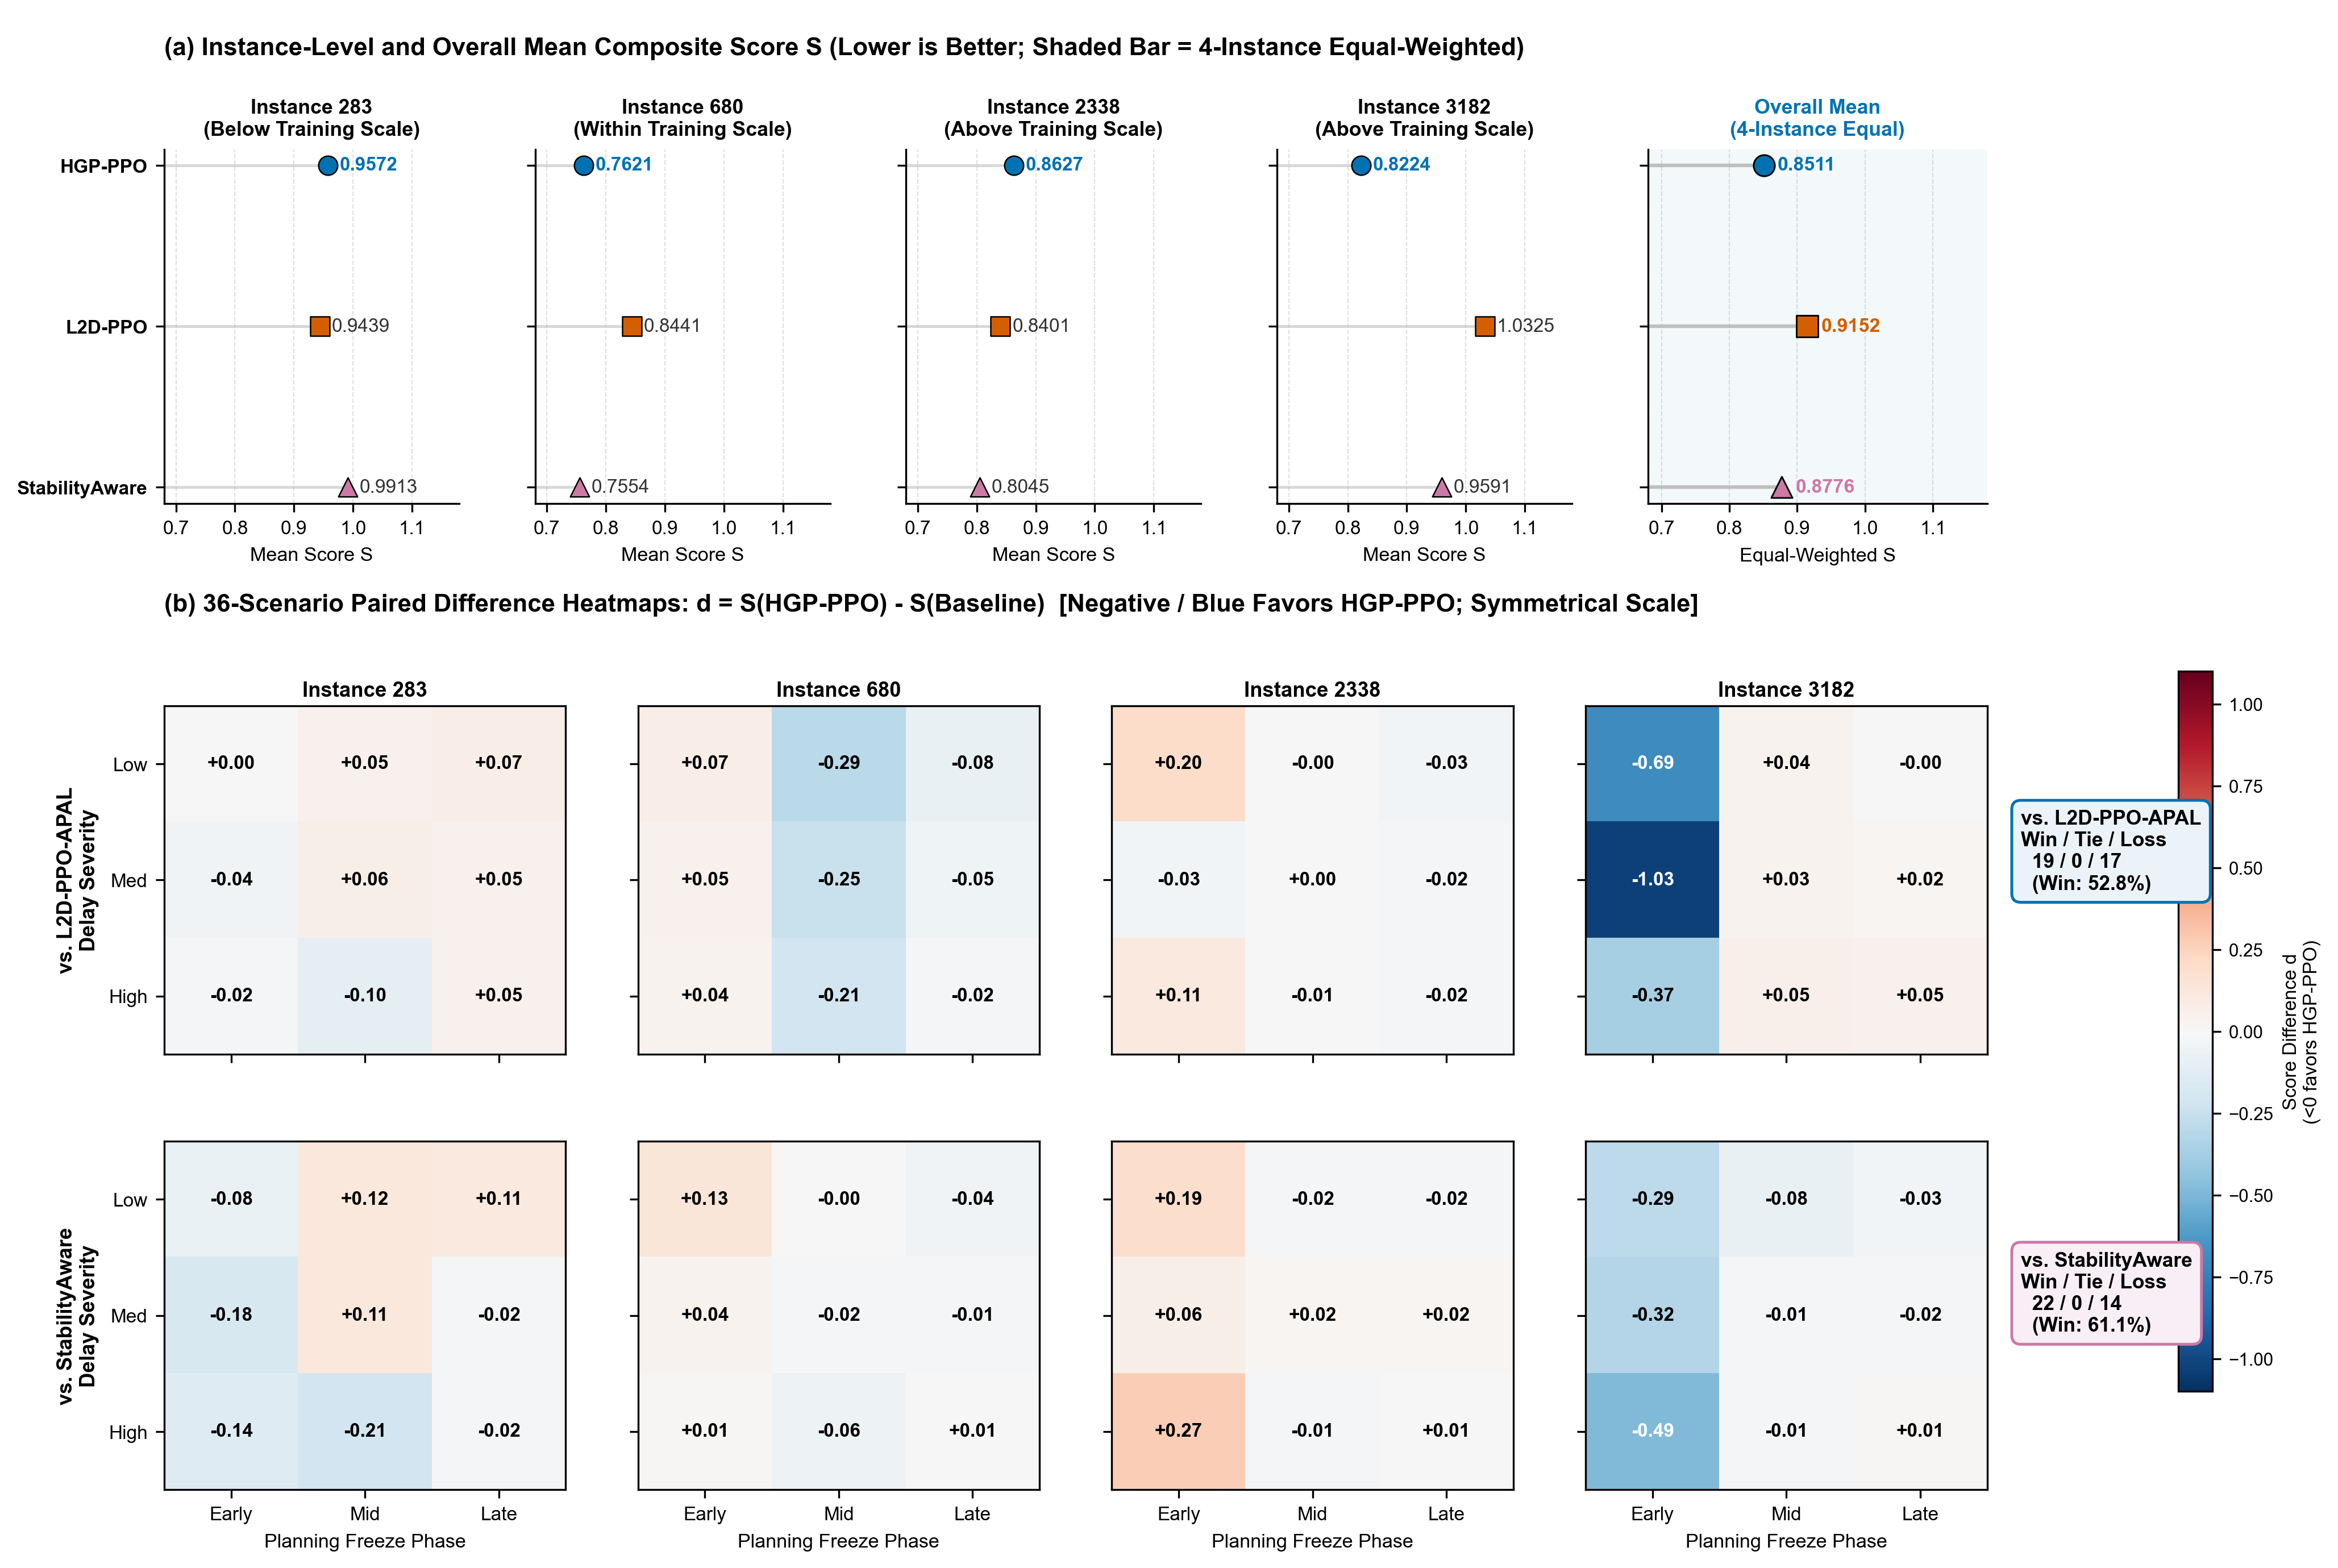
\includegraphics[width=0.92\textwidth,height=0.35\textheight,keepaspectratio]{figures/fig4_reschedule_scenarios_heatmap.png}
\caption{Paired-difference heatmaps for 36 template rescheduling scenarios under dynamic material delays and instance-level mean recovery scores. (a) Composite recovery scores $S$ for the four physical instance sizes and their equal-weight mean; lower is better. (b) Symmetric diverging heatmaps of paired score differences $d=S_{\mathrm{HGP}}-S_{\mathrm{Baseline}}$ between the proposed method and L2D-PPO-APAL or StabilityAwareRepair across 36 disturbance scenarios (four instances $\times$ three delay levels $\times$ three freeze timings). Blue indicates an advantage for the proposed method, and red indicates an advantage for the baseline. Win / Tie / Loss badges at the top summarize the pairwise comparisons.}
\label{fig:4}
\end{figure*}

\subsection{Online Runtime and Scalability}

Table~\ref{tab:runtime} and Fig.~\ref{fig:5} compare end-to-end online rescheduling runtimes. HGP-PPO executes forward inference in 8.02--123.60~s across the four scales. At the 3,182-operation scale, per-instance heuristic search requires 3,900--4,300~s ($\approx$65--72 minutes), whereas HGP-PPO finishes full-line plan repair in approximately 2 minutes (123.60~s), providing orders-of-magnitude acceleration for real-time shop-floor decision-making.

\begin{table}[!t]
\centering
\caption{End-to-End Online Rescheduling Runtime per Scenario (s)}
\label{tab:runtime}
\setlength{\tabcolsep}{4pt}
\renewcommand{\arraystretch}{1.05}
\begin{adjustbox}{max width=\columnwidth}
\begin{tabular}{@{}lrrrr@{}}
\toprule
\textbf{Method} & \textbf{283} & \textbf{680} & \textbf{2338} & \textbf{3182} \\
\midrule
\textbf{Proposed HGP-PPO} & \textbf{8.02} & \textbf{12.84} & \textbf{51.91} & \textbf{123.60} \\
BeamSearchRepair & 114.02 & 262.72 & 1787.00 & 3902.89 \\
IteratedGreedyRepair & 147.17 & 410.42 & 2416.80 & 4202.01 \\
SimulatedAnnealingRepair & 292.42 & 676.78 & 3445.39 & 4296.64 \\
\bottomrule
\end{tabular}
\end{adjustbox}
\par\smallskip
{\footnotesize Note: Single-scenario inference runtime excluding offline training and model loading.}
\end{table}

\begin{figure}[!t]
\centering
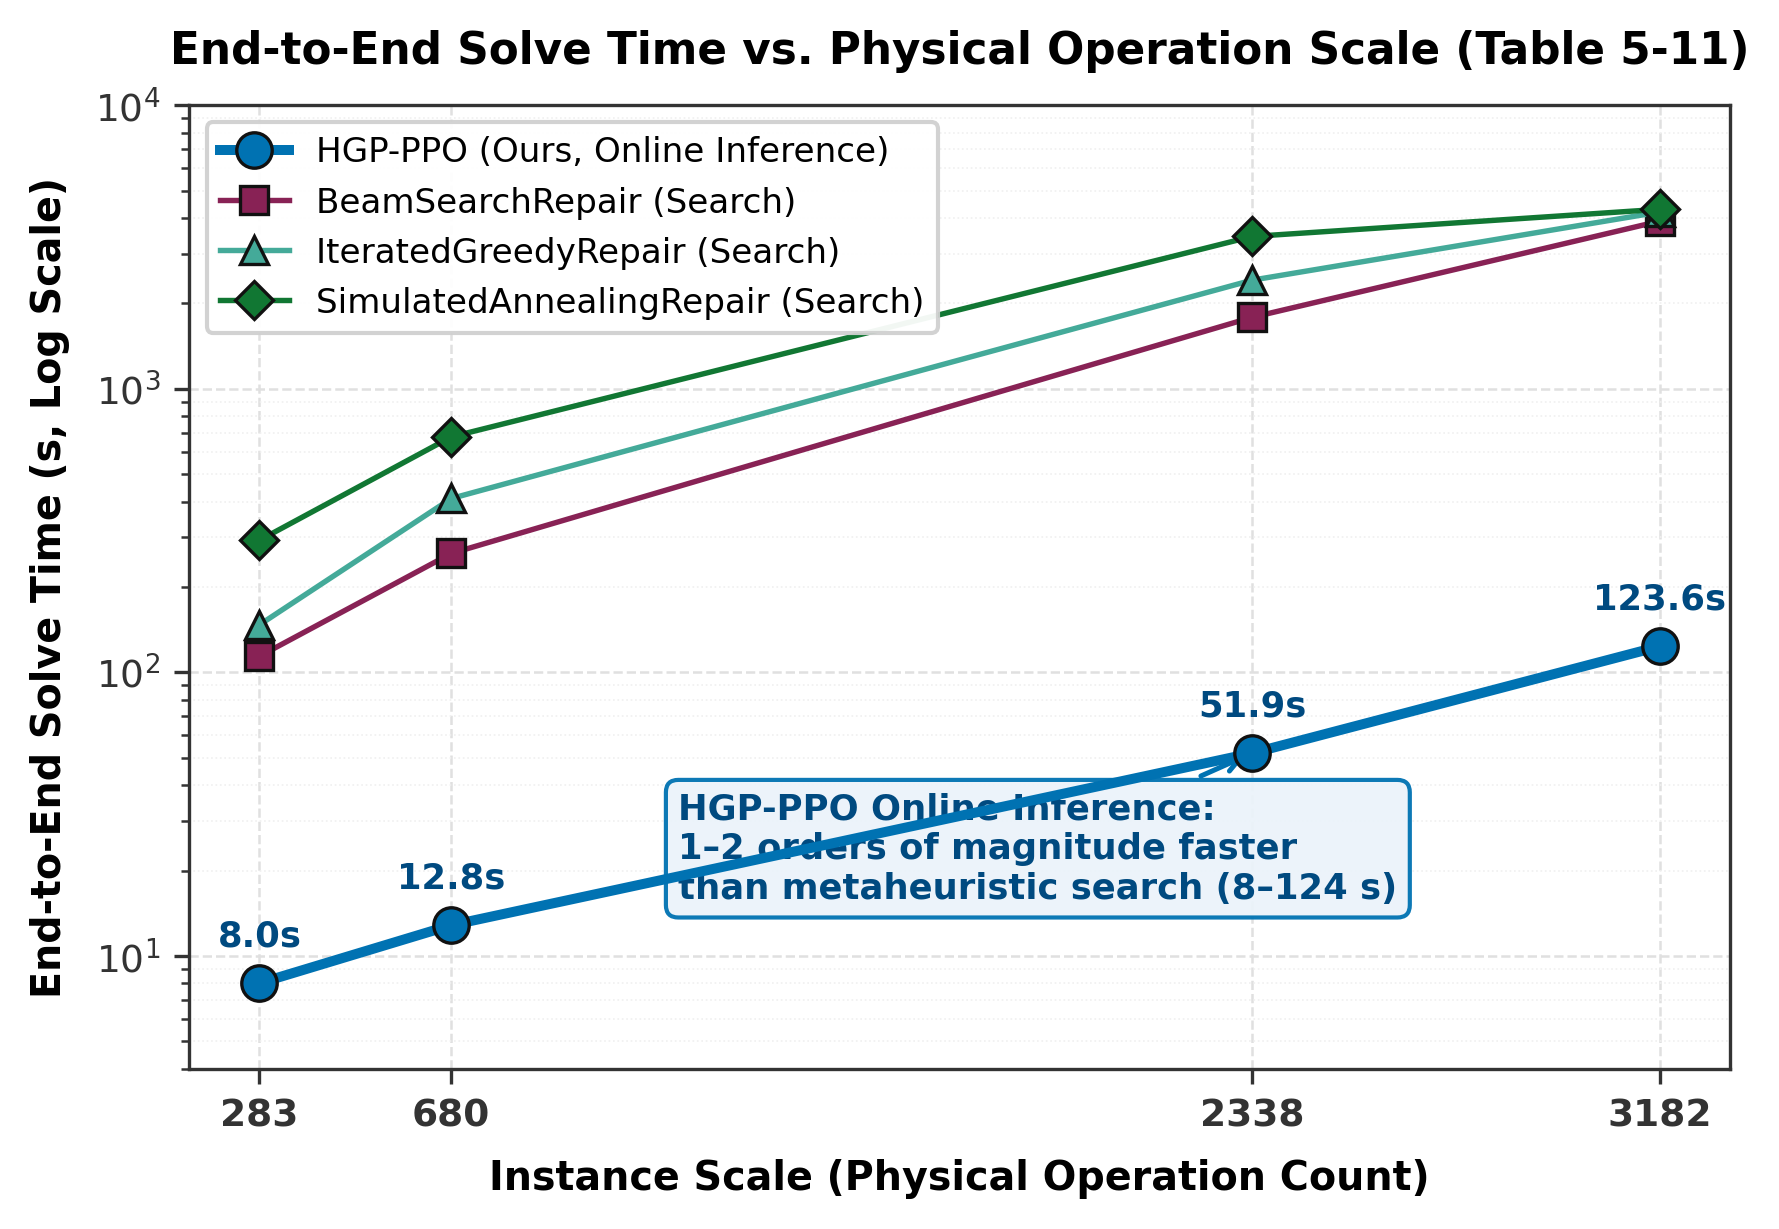
\includegraphics[width=\columnwidth]{figures/fig5_runtime_scalability.png}
\caption{End-to-end online rescheduling runtime and computational scalability across physical scales on a logarithmic axis.}
\label{fig:5}
\end{figure}

\section{Conclusions and Limitations}\label{sec:conclusions}

This paper has presented HGP-PPO, a heterogeneous graph reinforcement learning framework for joint scheduling and workforce allocation on aircraft pulsating assembly lines. The hierarchical operation--station--worker autoregressive pointer decoder and dynamic masks avoid explicit enumeration of complete teams, while endogenous worker--station binding coordinates workforce deployment with station workloads. For initial scheduling, a single locked policy is directly evaluated across 283 to 3,182 physical operations without instance-specific fine-tuning, achieving strong scale extrapolation and the lowest average makespan of 902.40~h. For rescheduling, the policy trained under the disturbance environment is evaluated across 36 locked material delay scenarios. All generated schedules in the designated test instances and scenarios pass model constraint validation, achieve a lower average composite recovery score with observable trade-offs among individual stability components, and require an average end-to-end plan repair runtime of approximately 2 minutes (123.60~s) per scenario on the largest 3,182-operation instance.

\textbf{Limitations and future work}: The present work investigates cyclic operation templates and plan-level cyclic template rescheduling under material readiness delays. While Proposition~1 establishes the physical feasibility of steady-state cyclic unfolding for a fixed template, the model does not explicitly simulate the physical transient dynamics and work-in-progress (WIP) buffer congestion that occur when shop-floor operations transition from an existing template to a newly rescheduled template with in-process aircraft at disparate completion stages. Furthermore, standard operation durations are assumed deterministic. Future investigations will incorporate continuous transient line simulations, stochastic operation durations, as well as worker fatigue and time-varying productivity.

\appendices

\section{Worker Pointer Architecture and Dynamic Features}\label{app:worker_pointer}

\textbf{Network layers and partial-team pooling}:
For the selected member sequence $\mathbf w_t^{(<r)}$, each member is projected via $\mathbf m_v = \mathbf W_{\mathrm{mem}}\mathbf h_v$. To achieve strict permutation invariance, partial-team state $\mathbf h_{\mathrm{team},t}^{(r)}$ is formed by symmetric Sum, Mean, and Max pooling:
\begin{center}
\begin{adjustbox}{max width=\columnwidth}
$\displaystyle
\mathbf h_{\mathrm{team},t}^{(r)} = \operatorname{LeakyReLU}\left(\mathbf W_{\mathrm{team}} \left[\sum_{v\in \mathbf w_t^{(<r)}} \mathbf m_v \,\|\, \frac{1}{\max(1, r-1)}\sum_{v\in \mathbf w_t^{(<r)}} \mathbf m_v \,\|\, \max_{v\in \mathbf w_t^{(<r)}} \mathbf m_v\right]\right).
$
\end{adjustbox}
\end{center}
For the initial member selection sub-step ($r=1$ where $\mathbf w_t^{(<1)}=\emptyset$), Sum, Mean, and Max pooling outputs are defined as zero vectors $\mathbf 0\in\mathbb R^d$, reducing the partial-team state to $\mathbf h_{\mathrm{team},t}^{(1)}=\mathbf 0$.

\newpage

Query $\mathbf q_t^{(r)}$ projects the concatenation of operation embedding, station embedding, global context, team state, macro pressure, skill consumption ratio, and selection progress:
\begin{center}
\begin{adjustbox}{max width=\columnwidth}
$\displaystyle
\mathbf q_t^{(r)}=\mathbf W_q\left[\mathbf h_{i_t}\,\|\,\mathbf h_{m_t}\,\|\,\mathbf g_t\,\|\,\mathbf h_{\mathrm{team},t}^{(r)}\,\|\,\mathbf P_t\,\|\,\mathbf c_t^{(r)}\,\|\,\mathbf{prog}_t^{(r)}\right]+\mathbf b_q,
$
\end{adjustbox}
\end{center}
where global context $\mathbf g_t = [\mathbf g_M \,\|\, \mathbf g_O \,\|\, \mathbf g_W] \in \mathbb R^{3d}$ strictly maintains the concatenation order of Section~\ref{sec:encoder}; macro skill pressure is $\mathbf P_t = [\mathbf P_t^{\mathrm{all}} \,\|\, \mathbf P_t^{\mathrm{near}}] \in \mathbb R^{10}$; skill consumption ratio is $\mathbf c_t^{(r)} = \mathbf C_t^{(r)} / \max(\mathbf S_t^{\mathrm{all}}, \varepsilon_s) \in [0,1]^5$ with cumulative committed headcount $\mathbf C_t^{(r)} = \sum_{v\in\mathbf w_t^{(<r)}} \mathbf H_v$; and selection progress is $\mathbf{prog}_t^{(r)} = \left[\frac{r-1}{q_{i_t}},\, \frac{q_{i_t}-(r-1)}{q_{i_t}}\right]^\top \in [0,1]^2$.

The candidate key combines candidate embedding, skill pressure exposure, and dynamic features:
\begin{equation}
\mathbf k_{w,t}^{(r)}=\mathbf W_k[\mathbf h_w\,\|\,\mathbf e_{w,t}]+\mathbf W_{\mathrm{eft}}\mathbf f_{w,t}^{\mathrm{eft},(r)}+\mathbf W_{\mathrm{sc}}\mu_{w,t}^{(r)},
\end{equation}
where skill pressure exposure $\mathbf e_{w,t} = [\mathbf H_w \odot \mathbf P_t^{\mathrm{all}} \,\|\, \mathbf H_w \odot \mathbf P_t^{\mathrm{near}}] \in \mathbb R^{10}$ remains fixed across selection sub-steps $r=1,\dots,q_{i_t}$ for operation $i_t$. Pointer scoring evaluates $\mathbf v_W^{\top}\tanh(\mathbf q_t^{(r)}+\mathbf k_{w,t}^{(r)})$, masked by $-10^4$ on invalid candidates.

\textbf{Global and near-term skill pressure}:
Let $R_{jk}\in\{0,1\}$ indicate whether operation $j$ requires skill $k$, $H_{wk}\in\{0,1\}$ indicate whether worker $w$ possesses skill $k$, and $\widetilde p_j$ be the normalized standard processing time. Let $\mathcal U_t\subseteq\mathcal O^+$ denote unscheduled physical operations, and let $\mathcal R_t\subseteq\mathcal U_t$ denote ready operations:
\begin{center}
\begin{adjustbox}{max width=\columnwidth}
$\displaystyle
D_{k,t}^{\mathrm{all}} = \sum_{j\in\mathcal U_t} R_{jk}\widetilde p_j q_j, \qquad D_{k,t}^{\mathrm{near}} = \sum_{j\in\mathcal R_t} R_{jk}\widetilde p_j q_j.
$
\end{adjustbox}
\end{center}
Let $\widetilde a_{w,t} = \exp(x_{w,t}^{\mathrm{log\_wait}}) - 1 \ge 0$ denote worker normalized wait time, and let $\mathcal W_t^q$ denote available workers not excluded by station queueing or binding restrictions:
\begin{center}
\begin{adjustbox}{max width=\columnwidth}
$\displaystyle
S_{k,t}^{\mathrm{all}} = \sum_{w\in\mathcal W} H_{wk}, \qquad S_{k,t}^{\mathrm{near}} = \sum_{w\in\mathcal W_t^q} H_{wk}\exp\!\left(-\frac{\widetilde a_{w,t}}{\tau_p}\right),
$
\end{adjustbox}
\end{center}
\begin{center}
\begin{adjustbox}{max width=\columnwidth}
$\displaystyle
P_{k,t}^h = \log\!\left(1 + \frac{D_{k,t}^h}{\max(S_{k,t}^h, \varepsilon_s)}\right), \qquad h\in\{\mathrm{all},\mathrm{near}\}.
$
\end{adjustbox}
\end{center}
Wait discounting temperature is set to $\tau_p=1.0$, and smoothing constant $\varepsilon_s=10^{-6}$ prevents division by zero.

\textbf{Dynamic EFT}:
With partial team wait $A_t^{(r-1)}$, cumulative efficiency $E_t^{(r-1)}$, station slot wait $\widetilde a_{m_t,t}$, and candidate baseline efficiency $\eta_w$, tentative completion time is:
\begin{center}
\begin{adjustbox}{max width=\columnwidth}
$\displaystyle
\widehat C_{w,t}^{(r)} = \max\!\left(A_t^{(r-1)}, \widetilde a_{w,t}, \widetilde a_{m_t,t}\right) + \frac{\widetilde p_{i_t}q_{i_t}}{\rho^{r-1}(E_t^{(r-1)}+\eta_w)}, \qquad \rho=0.95.
$
\end{adjustbox}
\end{center}
Across feasible candidate set $\mathcal F_{W,t}^{(r)}$, compute minimum completion $C_{\min,t}^{(r)}=\min_{u\in\mathcal F_{W,t}^{(r)}}\widehat C_{u,t}^{(r)}$, mean $\mu_{C,t}^{(r)}=\frac{1}{|\mathcal F_{W,t}^{(r)}|}\sum_{u\in\mathcal F_{W,t}^{(r)}}\widehat C_{u,t}^{(r)}$, and population standard deviation:
\begin{center}
\begin{adjustbox}{max width=\columnwidth}
$\displaystyle
\sigma_{C,t}^{(r)} = \sqrt{\frac{1}{|\mathcal F_{W,t}^{(r)}|} \sum_{u\in\mathcal F_{W,t}^{(r)}} \left(\widehat C_{u,t}^{(r)}-\mu_{C,t}^{(r)}\right)^2}.
$
\end{adjustbox}
\end{center}
The dynamic EFT feature consists of relative gap and clipped z-score:
\begin{center}
\begin{adjustbox}{max width=\columnwidth}
$\displaystyle
\mathbf f_{w,t}^{\mathrm{eft},(r)} = \left[ \operatorname{clip}\left(\frac{\widehat C_{w,t}^{(r)}-C_{\min,t}^{(r)}}{\widetilde p_{i_t}}, 0, 10\right),\, \operatorname{clip}\left(\frac{\widehat C_{w,t}^{(r)}-\mu_{C,t}^{(r)}}{\max(\sigma_{C,t}^{(r)}, 10^{-6})}, -10, 10\right) \right]^\top.
$
\end{adjustbox}
\end{center}
When $|\mathcal F_{W,t}^{(r)}|=1$, the standard deviation is zero, and denominator clamp $10^{-6}$ ensures numerical safety.

\textbf{Marginal skill scarcity}:
Candidate worker $w$'s marginal skill scarcity is:
\begin{center}
\begin{adjustbox}{max width=\columnwidth}
$\displaystyle
\begin{aligned}
\mu_{w,t}^{(r)} = \sum_{k\in\mathcal K} H_{wk}(1-R_{i_tk}) \Bigg[
&\log\!\left(1 + \frac{D_{k,t}^{\mathrm{all}}}{\max(S_{k,t}^{\mathrm{all}}-C_{k,t}^{(r)}-H_{wk},\varepsilon_s)}\right) \\
&- \log\!\left(1 + \frac{D_{k,t}^{\mathrm{all}}}{\max(S_{k,t}^{\mathrm{all}}-C_{k,t}^{(r)},\varepsilon_s)}\right) \Bigg]_+,
\end{aligned}
$
\end{adjustbox}
\end{center}
where $C_{k,t}^{(r)} = \sum_{v\in\mathbf w_t^{(<r)}} H_{vk}$ is the cumulative committed skill $k$ headcount across the prior $r-1$ sub-steps. The factor $(1-R_{i_tk})$ excludes skills required by operation $i_t$, quantifying the additional pressure on unrequired skill capacity and mitigating misallocation of multi-skilled workers on simple operations.

\section{Reproducibility Configuration and Metric Definitions}\label{app:reproducibility}

Table~\ref{tab:reproducibility} provides the key reproducibility settings.

\begin{table}[!t]
\centering
\caption{Key Reproducibility Hyperparameters}
\label{tab:reproducibility}
\setlength{\tabcolsep}{3pt}
\renewcommand{\arraystretch}{1.04}
\begin{adjustbox}{max width=\columnwidth}
\begin{tabular}{@{}llp{4.2cm}@{}}
\toprule
\textbf{Category} & \textbf{Parameter} & \textbf{Value / Configuration} \\
\midrule
Instances & Train / Dev / Locked test & 24 / 6 / 4 instances \\
Disturbances & Dev / Locked test & 54 / 36 (9 scenarios per instance) \\
Network & Architecture & 5 GATv2 layers, 4 heads, $d=128$ \\
Model size & Trainable parameters & $\approx$11.2 M \\
PPO & Learning rate / $\gamma$ / GAE $\lambda$ & $1.0\times10^{-4}$ / 0.999 / 0.9 \\
PPO & Epochs / clip range $\epsilon$ & 2 / $0.20\to0.10$ \\
Optimization & Optimizer / weight decay & ScheduleFree AdamW / $1.0\times10^{-4}$ \\
Gradients & Actor / Critic clip norms & 0.5 / 0.05 \\
Batching & Batch size / environments & 64 or 128 / 4 envs, grad accum 4 \\
Budget & Initial / rescheduling epochs & 60 epochs / 120 epochs (two stages) \\
\bottomrule
\end{tabular}
\end{adjustbox}
\end{table}

\textbf{Statistical metric definitions}:
\begin{enumerate}
\item \textbf{Interquartile mean (IQM)}: Arithmetic mean of the middle 50\% of scores after trimming the 25\% lowest and highest extremes.
\item \textbf{Average relative deviation (ARD)}: For method $m$ over scenario set $\mathcal S$ ($|\mathcal S|=36$):
\begin{equation}
\mathrm{ARD}_m = \frac{1}{|\mathcal S|}\sum_{s\in\mathcal S} \frac{S_{ms}-S_s^*}{S_s^*}\times100\%,
\end{equation}
where $S_s^*=\min_k S_{ks}$ is the \textbf{best score observed among all evaluated methods in scenario $s$}, rather than a theoretical optimum.
\item \textbf{Paired rank-biserial correlation ($r_{\mathrm{rb}}$)}: Nonparametric effect size for the Wilcoxon signed-rank test: $r_{\mathrm{rb}}=(W^+-W^-)/(W^++W^-)\in[-1,1]$.
\end{enumerate}

\begin{thebibliography}{30}
\bibitem{fang2021}
S.~Fang, M.~Liu, G.~Xian, \textit{et~al.}, ``Aircraft moving assembly line: Pulsating and continuous,'' \textit{Aeronaut. Manuf. Technol.}, vol. 64, no. 16, pp. 40--50, 2021.

\bibitem{bao2023}
Z.~Bao, L.~Chen, and K.~Qiu, ``An aircraft final assembly line balancing problem considering resource constraints and parallel task scheduling,'' \textit{Comput. Ind. Eng.}, vol. 182, p. 109436, 2023.

\bibitem{wang2024}
D.~Wang, F.~Qiao, L.~Guan, \textit{et~al.}, ``Human--machine collaborative optimization method for dynamic worker allocation in aircraft final assembly lines,'' \textit{Comput. Ind. Eng.}, vol. 194, p. 110370, 2024.

\bibitem{lu2019}
Z.~Lu, Y.~Ren, L.~Wang, \textit{et~al.}, ``A resource investment problem based on project splitting with time windows for aircraft moving assembly line,'' \textit{Comput. Ind. Eng.}, vol. 135, pp. 568--581, 2019.

\bibitem{becker2006}
C.~Becker and A.~Scholl, ``A survey on problems and methods in generalized assembly line balancing,'' \textit{Eur. J. Oper. Res.}, vol. 168, no. 3, pp. 694--715, 2006.

\bibitem{boysen2007}
N.~Boysen, M.~Fliedner, and A.~Scholl, ``A classification of assembly line balancing problems,'' \textit{Eur. J. Oper. Res.}, vol. 183, no. 2, pp. 674--693, 2007.

\bibitem{vieira2003}
G.~E.~Vieira, J.~W.~Herrmann, and E.~Lin, ``Rescheduling manufacturing systems: A framework of strategies, policies, and methods,'' \textit{J. Sched.}, vol. 6, no. 1, pp. 39--62, 2003.

\bibitem{hu2024}
J.-H.~Hu, J.-Y.~Zhu, Y.-N.~Sun, \textit{et~al.}, ``Network-based two-stage robust scheduling strategy for the aircraft assembly system with uncertain duration,'' \textit{Comput. Ind. Eng.}, vol. 188, p. 109911, 2024.

\bibitem{battaia2013}
O.~Batta\"ia and A.~Dolgui, ``A taxonomy of line balancing problems and their solution approaches,'' \textit{Int. J. Prod. Econ.}, vol. 142, no. 2, pp. 259--277, 2013.

\bibitem{bao2023b}
Z.~Bao, L.~Chen, and K.~Qiu, ``A surrogate-assisted heuristic approach for the joint optimization of resource allocation and scheduling of an aircraft final assembly line,'' \textit{J. Manuf. Syst.}, vol. 70, pp. 99--112, 2023.

\bibitem{fang2021flexible}
P.~Fang, J.-J.~Yang, Y.~Jiang, \textit{et~al.}, ``Flexible worker allocation in aircraft final assembly line using multiobjective evolutionary algorithms,'' \textit{IEEE Trans. Ind. Informat.}, vol. 17, no. 11, pp. 7468--7478, 2021.

\bibitem{liu2025}
M.~Liu, L.~Li, X.~Liu, \textit{et~al.}, ``A multi-pass heuristic for multi-skilled worker scheduling in aircraft final assembly line with variable duration,'' \textit{J. Syst. Eng. Electron.}, vol. 36, no. 6, pp. 1532--1547, 2025.

\bibitem{wen2026}
X.~Wen, H.~Liu, X.~Zhang, \textit{et~al.}, ``A Q-learning improved particle swarm optimization for aircraft pulsating assembly line scheduling problem considering skilled operator allocation,'' \textit{Comput. Mater. Contin.}, vol. 86, no. 1, pp. 1--27, 2026.

\bibitem{cappart2023}
Q.~Cappart, D.~Ch\'etelat, E.~B.~Khalil, \textit{et~al.}, ``Combinatorial optimization and reasoning with graph neural networks,'' \textit{J. Mach. Learn. Res.}, vol. 24, no. 130, pp. 1--61, 2023.

\bibitem{zhang2020}
C.~Zhang, W.~Song, Z.~Cao, \textit{et~al.}, ``Learning to dispatch for job shop scheduling via deep reinforcement learning,'' in \textit{Adv. Neural Inf. Process. Syst. (NeurIPS)}, vol. 33, 2020, pp. 1621--1632.

\bibitem{park2021}
J.~Park, J.~Chun, S.~H.~Kim, \textit{et~al.}, ``Learning to schedule job-shop problems: Representation and policy learning using graph neural network and reinforcement learning,'' \textit{Int. J. Prod. Res.}, vol. 59, no. 11, pp. 3342--3359, 2021.

\bibitem{wang2024flexible}
R.~Wang, G.~Wang, J.~Sun, F.~Deng, and J.~Chen, ``Flexible job shop scheduling via dual attention network-based reinforcement learning,'' \textit{IEEE Trans. Neural Netw. Learn. Syst.}, vol. 35, no. 3, pp. 3091--3102, 2024.

\bibitem{ai2025}
J.~Ai, F.~Qiao, J.~Liu, \textit{et~al.}, ``A graph-enhanced deep-reinforcement learning approach for the aircraft pulse assembly line balancing problem,'' in \textit{Proc. 2025 China Autom. Congr. (CAC)}, 2025, pp. 6623--6628.

\bibitem{wen2026b}
X.~Wen, H.~Zhang, W.~Yang, \textit{et~al.}, ``Research on a worker skill level-aware pulsating assembly scheduling method for aircraft based on the GIN-PPO algorithm,'' \textit{Comput. Ind. Eng.}, vol. 218, p. 112135, 2026.

\bibitem{vonder2007}
S.~Van~de~Vonder, E.~Demeulemeester, and W.~Herroelen, ``A classification of predictive-reactive project scheduling procedures,'' \textit{J. Sched.}, vol. 10, no. 3, pp. 195--207, 2007.

\bibitem{zhu2021}
H.~Zhu, Z.~Lu, C.~Lu, and Y.~Ren, ``A reactive scheduling method for disturbances in aircraft moving assembly line,'' \textit{Int. J. Prod. Res.}, vol. 59, no. 15, pp. 4756--4772, 2021.

\bibitem{chen2026}
B.~Chen, J.~Zhang, X.~Luo, \textit{et~al.}, ``A multi-agent graph attention deep reinforcement learning method for aircraft assembly dynamic scheduling,'' \textit{Adv. Eng. Inform.}, vol. 68, p. 104565, 2026.

\bibitem{brody2022}
S.~Brody, U.~Alon, and E.~Yahav, ``How attentive are graph attention networks?'' in \textit{Proc. Int. Conf. Learn. Represent. (ICLR)}, 2022.

\bibitem{smith1956}
W.~E.~Smith, ``Various optimizers for single-stage production,'' \textit{Nav. Res. Logist. Q.}, vol. 3, no. 1--2, pp. 59--66, 1956.

\bibitem{kelley1961}
J.~E.~Kelley, Jr., ``Critical-path planning and scheduling: Mathematical basis,'' \textit{Oper. Res.}, vol. 9, no. 3, pp. 296--320, 1961.

\bibitem{ow1988}
P.~S.~Ow and T.~E.~Morton, ``Filtered beam search in scheduling,'' \textit{Int. J. Prod. Res.}, vol. 26, no. 1, pp. 35--62, 1988.

\bibitem{ruiz2007}
R.~Ruiz and T.~St\"utzle, ``A simple and effective iterated greedy algorithm for the permutation flowshop scheduling problem,'' \textit{Eur. J. Oper. Res.}, vol. 177, no. 3, pp. 2033--2049, 2007.

\bibitem{kirkpatrick1983}
S.~Kirkpatrick, C.~D.~Gelatt, and M.~P.~Vecchi, ``Optimization by simulated annealing,'' \textit{Science}, vol. 220, no. 4598, pp. 671--680, 1983.

\bibitem{schulman2016}
J.~Schulman, P.~Moritz, S.~Levine, \textit{et~al.}, ``High-dimensional continuous control using generalized advantage estimation,'' in \textit{Proc. Int. Conf. Learn. Represent. (ICLR)}, 2016.

\bibitem{schulman2017}
J.~Schulman, F.~Wolski, P.~Dhariwal, \textit{et~al.}, ``Proximal policy optimization algorithms,'' \textit{arXiv preprint arXiv:1707.06347}, 2017.
\end{thebibliography}

\end{document}